\documentclass[10pt,a4paper, final]{report} % report
\usepackage[latin1]{inputenc}
\usepackage[left=3cm, right=2.5cm, top=2.5cm, bottom=2.5cm]{geometry}
\usepackage[english]{babel}
\usepackage{amsmath}
\usepackage{amsfonts}
\usepackage{amssymb}
\usepackage{graphicx}
\usepackage{verbatim}
\usepackage{hyperref}
\usepackage{booktabs}
\usepackage{todonotes} 
\usepackage{float}
%\usepackage{subfigure}
\usepackage{subfig}

%\usepackage{caption}
\DeclareCaptionFont{xipt}{\fontsize{9}{9}\mdseries}
\usepackage[font=xipt,labelfont=bf]{caption}

\usepackage{amsmath,amsfonts,amsthm,bm}
%\usepackage[usenames, dvipsnames]{color}

\linespread{1.5}

\title{Learning and Modulating Motor Commands using FORCE-trained Spiking Neural Networks}

\author{Carlo Alessi}

\begin{document}

\maketitle

\begin{abstract}
Supervised learning in networks of spiking neurons is efficiently carried out through a technique referred to as FORCE learning, at least for a certain range of frequency content in the teaching signals. As long as the teaching signals are limited to specific harmonics, FORCE can be efficiently used for learning and reproducing periodic signals \cite{nicola2017supervised}, for chunking input streams \cite{asabuki2018interactive}, implementing signal routing \cite{hoerzer2012emergence}, etc. The process however seems to break down when the teaching signals contain either low-frequency or very high-frequency components. This is due to the fact that the output of networks in the FORCE scheme is intimately bound to the intrinsic neuronal dynamics of these networks. This in turn currently restricts the applicability of the scheme to some toy examples, and prevents its more widespread use. 
In order to address these limitations, the following three questions are therefore of interest:
1) Can the FORCE scheme be adapted in order to learn sequences with low-frequency components, especially in the context of behaviourally-relevant motor tasks? 
2) Can the FORCE scheme be extended in order to learn sequences and replay them at speeds that differ from the teaching signal?
3) Can the FORCE scheme be linked to Reinforcement Learning to derive an error/reward signal to drive the weight update process (which is more biologically plausible), instead of using explicit target functions (that are not biologically plausible)? 
One possible path to explore in this framework is to consider whether the requirement of the FORCE scheme to use a chaotic, non-saturated regime as a starting point for the learning process can be relaxed, and what that entails in terms of network structure, readout schemes, temporal constants of neuronal dynamics and learning processes. Some practical solutions can be implemented that go in that direction, and applied to motor control in the HBP Neurorobotics Platform (with a proposed emphasis on control of arm movements).
\end{abstract}

\tableofcontents

\chapter{Background}
\label{cap:background}

\section{Introduction}
According to the International Federation of Robotics (IFR), robots play an important role in today's manufacturing industry\todo{cita summary IFR}. In the last decade there has been an increasing demand of robots in most of the industrial sectors, especially in the automotive and electronics industry. In particular, collaborative robotics is entering the market as the new frontier of industrial robotics, because it combines the high accuracy, speed and repeatability of robots with the flexibility and cognitive skills of humans \cite{villani2018survey}. The results are augmented worker productivity, stress and fatigue reduction.

\paragraph{Human-robot collaboration}
Collaborative robots (cobots) enable direct interaction between human operators and robots.
To obtain a successful and efficient human-robot interaction, several challenging problems must be solved: (i) motor control; (ii) safety issues; (iii) user interfaces; and (iv) user modeling.

Motor control for trajectory planning can be achieved using either standard methods based on control theory, or via more or less biologically plausible neurocontrollers.

Traditional industrial robots work confined into cages where humans are not allowed to enter. Conversely cobots are designed to collaborate with a human operator on the same area and task; therefore they need to be lightweight and be equipped with sensor avoidance sensors. A safe interaction must be guaranteed to prevent human-robot collisions and the risk of injuries.

Moreover, intuitive user interfaces must be properly designed, so that human operators can easily program and interact with the robot. Robots can be taught using several methods, such as systems based on augmented reality, programming by demonstration, etc.

Finally user modeling is needed to adapt the assistance provided by the cobot in order to maximise the operator's physical and cognitive well-being.


\paragraph{Project objectives}
In this project the focus in only on motor control by means of a neural network. The aim is to use a single neural network to learn a set of primitives that would allow an industrial robotic arm to reach several points in a workspace and return to a home position, operating at different velocities (accelerating and decelerating on demand).

advantages of proposed approach (implementation on neuromorphic hardware, see ipad)

\paragraph{Possible real-world applications}
The results of this project could find a direct application in industrial scenarios where (i) robots are used in assembly lines or (ii) collaborate with a human operator.

For the assembly line, a robot operating by a conveyor belt could adapt its velocity according to the velocity of the conveyor belt. For the human-robot collaboration, the robot could adapt to the human speed.

interpolazione buona per coprire tutta l'area di uno scaffale o di un piano da lavoro.

- interpolazione molto importante perche non devi imparare ogni singola posizione. buona
  capacita di generalizzazione

\paragraph{Thesis outline}
The outline of the thesis is as follows. 

The remaining of \autoref{cap:background} covers the background material. The necessary robotics fundamentals are summarized in \autoref{sec:robotics_foundamentals}. 
Section \ref{sec:izhikevich_model} reviews the Izhikevich neuron model, which is one of the main building blocks of the neural network used. Section \ref{sec:FORCE_method} describes the main features and functioning of the FORCE learning scheme, while \autoref{sec:related_work} reviews some applications of FORCE training in learning complex natural signals, as well as some relevant contributions to motor control using neurocontrollers.

In \autoref{cap:method} the methodologies adopted in the project are explained in detail. The datasets used in the experiments are described in \autoref{sec:datasets}. \todo{finisci}

The results are reported in \autoref{cap:result}. \todo{finisci}

The results are discussed in \autoref{cap:discussion}. \todo{finisci}

\autoref{cap:conclusion} concludes with a summary of the main findings and an insight for future work.

\section{Robotics Foundamentals}
\label{sec:robotics_foundamentals}
links, joints, DH parameters, forward and inverse kinematics, how can the IK be solved, IK challenges, PID control (?), neurocontrollers

\section{The Izhikevich model}
\label{sec:izhikevich_model}
The Izhikevich model \cite{izhikevich2003simple} is one of the most widely used models of spiking neurons because it combines the biological plausibility of the Hodkin-Huxley model and the computational efficiency of Integrate-and-Fire neurons. In this project it was used a variant of the model proposed by Nicola \& Clopath in \cite{nicola2017supervised}.
The model is composed of two components: (i) a two-dimensional system of ordinary differential equations \eqref{eq:izhikevich_model}, which models the sub-threshold behaviour of the system and generates the upstroke of the action potential; (ii) an after-spike reset mechanism \eqref{eq:reset_mechanism}, which generates the downstroke of the action potential.

\begin{subequations}
\label{eq:izhikevich_model}
\begin{align}
C \dot v &=  k(v - v_{rest}) (v - v_{threshold}) - u + I \label{eq:izikevich_membrane}\\
\dot u &= a(b(v - v_{rest}) - u)
\end{align}
\end{subequations}

\begin{equation}
if\ v \geq v_{peak}\ then
\begin{cases}
v \leftarrow c \\
u \leftarrow u + d\\
\end{cases}
\label{eq:reset_mechanism}
\end{equation}

The two variables of the model are the membrane potential $\bm{v}$ ($mV$), and the adaption/recovery variable $\bm{u}$ ($pA$), which allows for spike frequency adation, and represents the effect of slow current on the spike generation.

The model presents a wide variety of parameters.
\begin{itemize}
\item $\bm{C}$ $(pF)$, membrane capacitance;
\item $\bm{v_{rest}}$ $(mV)$, resting membrane potential;
\item $\bm{v_{threshold}}$ $(mV)$, voltage threshold when $b=0$ and $I = 0$;
\item $\bm{I}$ $(pA)$, injected or synaptic current;
\item $\bm{v_{peak}}$ $(mV)$, voltage peak (i.e. spike cutoff value);
\item $\bm{k}$ $(nS/mV)$, gain on $v$; \todo{cambia il nome del parametro k, perche gia usato per il numero di dimensioni del segnale}
\item $\bm{a}$ $(ms^{-1})$, time constant of the adaption current;
\item $\bm{b}$ $(nS)$, sensitivity of the adaption current $u$ to subthreshold fluctuations of the membrane potential $v$;
\item $\bm{c}$ $(mV)$, post-spike reset value of the membrane potential;
\item $\bm{d}$ $(pA)$, post-spike additive value to the recovery variable $u$. 
\end{itemize}
\todo{maybe make a table with parameter-units-description}

The parameter $k >0$ is a scaling factor that controls the action potential up-swing \cite{dur2012network}. It affects the value of $\dot{v}$ and hence the spike width. It is important for determining the half width of the action potential. Smaller values of $k$ give smaller half widths. 

The parameter $b$ describes how sensible is $u$ to subthreshold oscillations of $v$. Greater values of $b$ couple $v$ and $u$ more strongl, resulting in possible subthreshold oscillations and low-threshold spiking dynamics. \todo{what does it mean?} 
The sign of $b$ determines whether the effect of $u$ is amplifying ($b < 0$) or resonant ($b >0$).

The voltage reset value $c$ is designed to model the effect of fast high-threshold $K^+$ conductances. The appropriate choice of this parameter will help to obtain a suitable fast post-hyperpolarization.

The value $d$ is added to the recovery variable $u$ after a spike occurs. It describes the total amount of outward minus inward currents activated during the spike, which affects the after-spike behaviour. This parameter, together with $a$, determines how much spike frequency adaption the model exhibits. 

Note that both $u$ and $I$ are currents and in \eqref{eq:izikevich_membrane} they have opposite sign ($-u$ and $+I$). Therefore they can potentially balance each other out. Moreover the negative feedbak that $u$ has on the membrane potential $v$, combined with the after spike reset ($u \leftarrow u + d$), mean that both the value and sign of $d$ influence the spike frequency adaption. 

In particular, when $d < 0$, the variable $u$ tends to become negative. Therefore the current $-u$ will be exitatory. As a result the network could spike at a higher rate (i.e. spike facilitation). Moreover the more it spikes, the more it is easy to produce ulterior spikes. Conversely when $d > 0$, the current $u$ will become inhibitory. In the special case where $d = 0$ the network is neither facilitated or discouraged to spike.

At each time $t$, the discretized evolution of the system dynamics is given by:

\begin{align}
v(t+1) &= v(t) + \delta t \cdot [( k(v(t) - v_{rest}) (v(t) - v_{threshold}) - u(t) + I)]/C\\
u(t+1) &= u(t) + \delta t \cdot a[b(v(t) - v_{rest}) - u(t)]
\end{align}

The value $\bm{\delta t}$ is the integration time constant. If at time $t$ a spike occurs, the variables $\bm{v}$ and $\bm{u}$ are reset according to \eqref{eq:reset_mechanism}.

\section{The FORCE method}
\label{sec:FORCE_method}
The FORCE training method originated in the field of reservoir computing, and was first proposed by Sussillo et Al. in \cite{sussillo2009generating}.
It is used to modify the synaptic strengths of an artificial neural network, either external or withing the model, to change chaotic spontaneous activity into a wide variety of desired patterns.
The method is widely applicable because any multi-dimensional dynamical system can be used as a reservoir, guiding its dynamics using and error signal. Therefore FORCE can be used with many network type to solve many task. Unlike other techniques, the target behaviour does not have to be specified as a closed form differential equation for training. All that is required for training is a supervisor to provide an error signal.

A variant of the original FORCE method, proposed by Nicola\&Clopath in \cite{nicola2017supervised}, is described below. 

%assuming the network architecture in \autoref{fig:network_architecture}, which will be subject to further modifications during this project, and that the network output has dimension $m$.

\paragraph{Network architecture}
The newtork architecture is a Recurrent Neural Network (RNN) composed by a reservoir of Izhikevich neurons, a linear layer of readout units, and a feedback channel that connects the output of the readouts back into the reservoir, see \autoref{fig:network_architecture}.

\begin{figure}[H]
\centering
\includegraphics[width=\columnwidth]{images/FORCE_rete.png}
\caption{Network architecture. Example of a reservoir with $N=8$ Izhikevich neurons and $k=1$ readout unit.}
\label{fig:network_architecture}
\end{figure}

\paragraph{Network weights}
In the FORCE method, the weight matrix $\omega$ is decomposed by a static weight component $\bm{\omega^0}$, a learned decoder $\bm{\phi}$, and a static matrix $\bm{\eta}$:

\begin{equation}
\omega = G \omega^0 + Q \eta \phi^{\intercal}
\label{eq:force_matrix}
\end{equation}

The term $\bm{\omega^0} \in \mathbb{R}^{N \times N}$ is a sparse and static weight matrix that determines the connectivity of the neurons inside the reservoir, and induces chaos in the network. The chaos is balanced by the constant $\bm{G}$. Each element $\omega_{ij}$ is the weight of the synaptic connection between the pre-synaptic neuron $j$ and the post-synaptic neuron $i$. 

The component $\bm{\phi} \in \mathbb{R}^{N \times k}$ is the weight matrix of the readout layer, which serves as a linear decoder of the network dynamics. The values of $\bm{\phi}$ are learned using a supervised learning method called Recursive Least Squares (RLS).

The static matrix $\bm{\eta} \in \mathbb{R}^{N \times k}$ encodes the output of the readout layer back into the reservoir, and defines the tuning preference of the neurons. The constant $\bm{Q}$ balances the effects of the decoder. 

\paragraph{Network output}
The network output is defined as a weighted sum of the network activities, and determines the task that the network performs. The network activities at time $t$ are specified by a column vector $\bm{r(t)}$, which correspond to the firing rate of each of the $N$ neurons of the reservoir. 

The task of the network is to approximate the dynamics of a $k$-dimensional teaching signal, $\bm{x(t)} \in \mathbb{R}^k$, with the following approximant

\begin{equation}
\hat{x}(t) = \phi^\intercal r
\label{eq:network_output}
\end{equation}

\paragraph{Recursive Least Squares update}
FORCE learning requires a learning rule that rapidly reduces the magnitude of the error to a small value, and then keeps it small while the readout weight vector converges to a solution that can maintain the error small post training. The authors in \cite{sussillo2009generating} reported that the Recursive Least Squares (RLS) rule is a suitable and very powerful method for FORCE learning.

RLS is a weight update rule that minimizes the squared error between the
network dynamics $\bm{\hat{x}(t)}$ and the target dynamics $\bm{x(t)}$ during training. The training process is considered successful if the network can well approximate the target dynamics post training. Every $\Delta t$, the readout weights are updated with the following rule\footnote{Note that the time interval that pass from one weight update to the next is greater than the integration time constant, i.e. $\Delta t > \delta_t$.}

\begin{equation}
\phi(t) = \phi(t - \Delta t) - e(t) P(t) r(t)
\label{eq:RLS_readout_weights_update}
\end{equation}

where $\bm{e(t) = \hat{x}(t) - x(t)}$ is the error between the approximant and desired dynamics, and $\bm{r(t)} \in \mathbb{R}^N$ is the vector of firing rates of the neurons. The matrix $\bm{P(t)}$ is the network estimate for the inverse of the correlation matrix of the neuron firing rates $\bm{r}$, plus a regularization term:

\begin{equation}
P(t) = (\sum_t r(t) r(t)^\intercal + \lambda I_N)^{-1}
\end{equation}

The parameter $\lambda$ acts as a regularization parameter and controls the rate of
the error reduction, while $\bm{I_N}$ is the $N \times N$ identity matrix.
The matrix $\bm{P}$ is also updated at the same time as the weights, according to the rule:

\begin{equation}
P(t) = P(t - \Delta t) - \frac{P(t - \Delta t) r(t) r(t)^\intercal P(t - \Delta t)}{1 + r(t)^\intercal P(t - \Delta t) r(t)}
\end{equation}

The weight update rule \eqref{eq:RLS_readout_weights_update} can be viewed as a standard delta-type rule, but instead of having a single scalar learning rate (e.g. as in Gradient Descent), it uses multiple learning rates given by the matrix-vector product $\bm{P(t) r(t)}$. The parameter $\lambda$, also functions as a learning rate, and should be adjusted depending on the particular target function being learned. Small $\lambda$ values result in fast learning, however weight changes could be so rapid that learning becomes unstable. Conversely if $\lambda$ is too large, the FORCE algorithm may not be able to keep the network output close to the desired dynamics for a long enough time, causing the learning to fail. Moreover the author report that for a correct functioning the learning rate should be subject to the constraint $\lambda \ll N$\cite{sussillo2009generating}. Values in the interval $[1,100]$ performs well in practice.

\paragraph{Injected Current}
FORCE can make the network learn a single target $\bm{x}$ in the absence of any external input, but in the general case, different outputs depend on different inputs. 

The spikes are filtered by a double exponential filter of the form

\begin{align}
\dot{r}_j &= - \frac{r_j}{\tau_d} + h_j\\
\dot{h}_j &= - \frac{h_j}{\tau_r} + \frac{1}{\tau_r \tau_d} \sum_{t_{jk} < t} \delta(t - t_{jk})
\end{align}

where $\bm{\tau_r}$ is the synaptice rise time, $\bm{\tau_d}$ is the synaptic delay time, and $\bm{t_{jk}}$ is the time of the $k$-th spike fired by neuron j. 

The synaptic currents are given by the equation:

\begin{equation}
s_i(t) = \sum_{i=1}^N \omega_{ij} r_j
\end{equation}

\todo{understand double exponential filter and what is IPSC.}
... ... ... ...

The current is
\begin{equation}
I = IPSC + \eta \hat{x}(t- \delta_t) + I_{BIAS}
\end{equation}

\paragraph{Feedback}
\todo{some observation about the feedback channel}

\paragraph{Error reduction}
Most learning algorithms repeatedly modify the weights in order to gradually reduce the error, which is quite large at the beginning. This process goes on until the weights converge to a solution where the vector changes minimally, so that the training can be terminated. However, in FORCE training the error magnitudes become small from the first weight update, and the goal is to keep it small throughout the training process. 

\paragraph{Weights initialization}
The static sparse matrix $\bm{\omega^0}$ is drawn from a normal distribution with mean $\mu = 0$, and standard deviation $\sigma = 1/\sqrt{Np}$, where $p$ is the probability connection of the matrix. 
The encoding variables, $\bm{\eta_i} \in \mathbb{R}^k$, are drawn randomly and uniformly from $[-1,1]^k$ , where $k$ is the dimensionality of the teaching signal.
The readout weights are initialized as $\bm{\phi(0) = 0}$.
The matrix $\bm{P}$ is initially estimated with $\bm{P(0)} = \lambda^{-1} \bm{I_N }$, where $\lambda$ is a constant parameter.

\section{Related Work}
\label{sec:related_work}

\subsection{FORCE training to learn multiple signals}
The FORCE method was first proposed by Sussillo et Al. in \cite{sussillo2009generating}. They showed that using FORCE learning it is possible to construct various network architectures that can produce (i) a wide variety of complex output patterns, (ii) input-output transformations that require memory, (iii) multiple outputs that can be switched by control inputs, and (iv) motor patterns matching human motion capture from data. 

\paragraph{4-bit memory}
As an example, they designed a network that functions as a 4-bit memory that is robust to input noise. The network has 8 inputs that randomly connect to neurons in the network, and are functionally divided into pairs. The input values are held at zero except for short pulses to positive values that act as ON and OFF commands for the four readout units. Post FORCE learning, the inputs are correctly mapped to the corresponding output, with little interference between inputs and inappropriate outputs. In order to have a functioning model, the network is required to have 16 point attractors, one for each of the $4^2$ possible combinations of the four outputs. Moreover the network must be able to transition between these attractors in response to a pulse to one of the inputs.

\paragraph{Motion capture}
The authors  also demonstrated that FORCE learning can be used to train a single chaotic recurrent network to generate multiple, high-dimensional, nonperiodic patterns that resemble complex human motions. They used a dataset from the CMU motion capture library, which consists of 95 joint angles trajectories for walking and running activity, measured over hundreds of time steps. The data was obtained from human subjects performing these activities while wearing a suit that permits the measurement of the joint angles. The 95 joint angles were predicted by 95 readouts. To cope with the nonperiodicity of the motions, they introduced static control inputs to initialize the network prior to starting the running or walking motions. The control inputs were also used to switch between the different activities.

\subsection{High-dimensional temporal signals improve FORCE learning}
The FORCE method has been successfully adopted to learn oscillators. In \cite{nicola2017supervised} it was shown that FORCE training can be aided to learn more complex behaviours by the so called high dimensional temporal signals (HDTS). The HDTS, inspired by the clock-like input pattern that songbirds use for learning and replay, discretizes time by segregating the neurons into assemblies that fire at specific time intervals. 

The HDTS can be (i) \textit{internally generated} by a separate HDTS network, or (ii) \textit{externally generated} and directly fed as input into and encoding and replay network (see \autoref{fig:HDTS}). Nicola \& Clopath explored the benefit of HDTS in learning complex signals such as a portion of a song and a movie scene, using either internally or externally generated HDTS. 

\begin{figure}
\centering
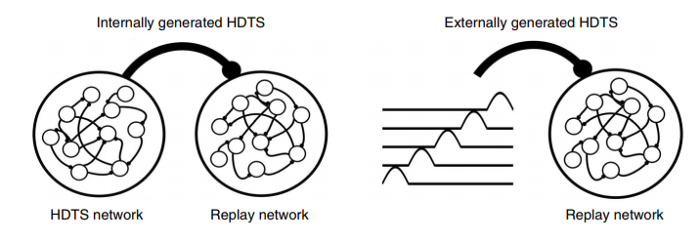
\includegraphics[width=1\textwidth]{images/HDTS}
\caption{Internally and externally generated HDTS. (figure taken from \cite{nicola2017supervised})}
\label{fig:HDTS}
\end{figure}

\paragraph{Learn a song fragment}
They FORCE trained an HDTS network of Izhikevich neurons to internally generate its own HDTS, while simultaneously also training a replay network to reproduce the first bar of Ode to Joy. The supervisor consisted of 5 notes, plus 16 other components of the HDTS which correspond to a sequence of 16 pulses that partition time. The networks learned both the HDTS and the song, with less training time and greater accuracy than without HDTS. They also succeded in learning the first four bars of the song (corresponding to 16 seconds) with a 64-dimensional HDTS.

\paragraph{Learn a movie scene}
To investigate if HDTS would help to learn natural high-dimensional signals, they trained a network of Izhikevich neurons to learn a movie scene of 8 seconds. The high-dimensional supervisor consisted in the evolution of the 1920 pixels of the frame. The training of the replay network was successful for both internally and externally generated HDTS.

They observed that the HDTS inputs were necessary both for training and replay. Without HDTS, the network could still replay the individual frames from the movie scene; however the order of scenes was incorrect and appeared chaotic. Moreover, decreasing the HDTS amplitude yield a steady decrease in replay performance. Also, by observing the histogram of spike times in the replay network, they noticed that the HDTS conferred a strong $4Hz$ modulation (the histogram can be interpreted as the mean network activity). Removing the HDTS, the mean network activity displayed a much slower oscillation ($\approx 2 Hz$), which corresponded to a sharp decline in replay performance, as the scenes were no longer played in chronological order.

\paragraph{Frequency and amplitude of HDTS}
They wondered how the frequency and amplitude of HDTS would affect the learning performance of a network. They found that an optimal input frequency was located in the interval $8-16 Hz$, for large regions of parameter space, which was robust to different neural parameters.

\paragraph{Accelerated and reverse replay}
Several studies speculated that compressed of reversed replay of an event might be important for memory consolidation \todo{(cite studies?)}. Thus they wondered if networks trained with an HDTS could replay the scene in accelerated time by compressing the HDTS post-training. They compressed the external HDTS after training, and uncovered that the network was able to replay the movie scene in compressed time up to a compression factor of 16x (correlation $r > 0.8$). The accuracy sharply dropped for further compression.
The effect of time compression on the mean activity was to introduce higher frequency oscillations\todo{use a low-pass filter to smooth?}. The frequency of these oscillations scaled linearly with the amount of compression. However, with increasing compression frequency, large waves of synchronized activity also emerged in the mean population activity.

Reverse replay was also successfully obtained by reversing the order in which the HDTS components were presented to the network (correlation $r=0.9$). The authors reported that the loss in accuracy was due to the fact that the temporal dynamics of the network is not reversed within a segment of the HDTS\todo{how to counter this?}. Therefore the network could generalize robustly to accelerated and inverse replay, despite not being trained to do so.

The key findings of \cite{nicola2017supervised} regarding HDTS can be summarized as follows:

\begin{itemize}
\item HDTS can make FORCE training faster, more accurate, and more robust to learn longer signals.
\item HDTS inputs facilitate both learning and spontaneous replay of high-dimensional signals.
\item a network trained with HDTS can repeat the signals in accelerated time or in inverse order by compressing or reversing the HDTS.
\end{itemize}

\subsection{Robot control via artificial neural networks}
In this section some proposed solutions to robot control using artificial neural networks are reviewed.

\paragraph{I.}
A simple but valuable example was proposed by Duka in \cite{duka2014neural}. The author investigated the use of a feed-forward neural network to solve the IK problem for a three-link simulated robotic arm. 
The hypothetical robotic arm was composed by three movable links $l_1$, $l_2$, $l_3$, of the same size $l_1 = l_2 = l_3 = 2$ that operate within a plane. The links are connected by three rotational joints, $q_1$, $q_2$, $q_3$, which have the axes of rotation perpendicular to the plane where the links lie. The joints movements were respectively limited by the intervals 

\begin{equation}
q_1 \in [0, \pi], \qquad q_2 \in [-\pi, 0], \qquad q_3 \in [-\frac{\pi}{2}, \frac{\pi}{2}]
\label{eq:duka_joint_values}
\end{equation}


The coordinate position $P_E = (X_E, Y_E)$ of the end-effector, with respect to the reference system located to the base of the robot $O_{X_0 Y_0}$, is defined by the following forward kinematics equations

\begin{align}
X_E &= l_1 \cos(q_1) + l_2 \cos(q_1 + q_2) + l_3 \cos(q_1 + q_2 + q_3)\label{eq:duka_forward_kinematics}\\
Y_E &= l_1 \sin(q_1) + l_2 \sin(q_1 + q_2) + l_3 \sin(q_1 + q_2 + q_3)\nonumber
\end{align}

The orientation $\Theta_E$ of the end-effector, described by the angle of rotation of the reference system attached to the end-effector $O_{X_E Y_E}$ relative to $O_{X_0 Y_0}$, is defined as 

\begin{equation}
\Theta_E = q_1 + q_2 + q_3
\end{equation}

The task of the robotic manipulator was to perform a circular trajectory in its workspace. The points in this trajectory were defined by the equation of a circle of radius $r$,  centred in $(x_c, y_c)$, parameterized by $\varphi$

\begin{align}
X_d &= x_c + r \cos \varphi \nonumber\\
Y_d &= y_c + r \sin \varphi\\
\varphi &\in [0, 2 \pi] \nonumber
\end{align}

The point $P_d = (X_d, Y_d)$ corresponds to the desired position of the end-effector.
The desired orientation $\Theta_d$ of the end-effector is expressed by the angle between the positive x-axis and the line that connects $O_{X_0 Y_0}$ to a point on the circle trajectory

\begin{equation}
\Theta_d = \arctan \frac{Y_d}{X_d}
\end{equation}

The training data for the neural network was generated by sampling 1000 random joint angle values uniformly over the intervals defined in \eqref{eq:duka_joint_values}. From each sampled configuration of joint angle values $(q_1, q_2, q_3)^\intercal$, the corresponding end-effector pose $(X_E, Y_E, \Theta_E)^\intercal$ was computed with the forward kinematics equations defined in \eqref{eq:duka_forward_kinematics}. To counter the fact that for the same end-effector pose $(X_E, Y_E, \Theta_E)^\intercal$ the IK problem has multiple solutions $(q_1, q_2, q_3)^\intercal$, the author removed duplicates in order to obtain a unique cartesian-joint space mapping.
Before training, a final preprocessing step was applied to scale the entire dataset to the interval $[-1, 1]$.

The neural network was trained to map $(X_E, Y_E, \Theta_E)^\intercal$ to $(q_1, q_2, q_3)^\intercal$ using the Levenberg-Marquardt algorithm. The dataset was divided according to the following partition percentages: 70\% training set, 15\% validation set, 15\% test set. The performance was evaluated computing the mean squared error between the network output and the desired output. The error reduced to the order of $O(10^{-3})$ in circa 10 training epochs. The network architecture consited in 3 input neurons, 3 linear output neurons, and one hidden layer with 100 tanh neurons.
\todo{conclude paragragh}

\paragraph{II.}
Another solution based on multilayer perceptrons to solve the inverse kinematics problem was proposed by Aggarwal et Al. in \cite{aggarwal2014use}, with a focus on the prediction of singularity zones. 

They used the PUMA 560 robot manipulator, which has six degrees of freedom. The first three joints determine the end-effector position, while the last three joints determine the end-effector orientation. 
The Forward Kinematics of the robot was computed using homogeneous transformation matrices $^{(i-1)}A_i$, defined by the D-H parameters of the PUMA 560 manipulator. A dataset of 1000 samples was constructed using the values of the joint angles $\theta_1, \ldots, \theta_6$, and the corresponding cartesian coordinates of the end-effector $(X_E,Y_E,Z_E)$, which were computed from $^0A_6$ using unique combinations of the joint angle ranges.

As above, the neural network was trained to map cartesian coordinates to joint angles, minimizing the mean square error using the Levenberg-Marquardt learning rule. The network architecture consited in three input neurons, one hidden layer with 30 sigmoid neurons, and six linear output neurons. The dataset was partitioned in 70\% training set, 15\% validation set, and 15\% test set. The test set was used to measure the network performance on cartesian points where the singularity condition was satisfied. In this set, it was obtained a 1.32 MSE.
Moreover, it was observed that singularity zones were located throughout the robot workspace. They reported that this was due to the fact that the PUMA 560 manipulator assumes a singularity condition when $\theta_5 = 0$ radians.

\paragraph{III.}
A slightly different approach for robot control was studied by Bouganis \& Shanahan in \cite{bouganis2010training}. They presented a Spiking Neural Network architecture that autonomously learns to control a 4-DoF robotic arm in the three-dimensional space, after an initial period of \textit{motor babbling}\footnote{\textit{Motor babbling} is the process of repeatedly performing small random motor movements for a short duration, that tries to mimic human-like cognition and learning. The robot performing motor babbling can autonomously develop an internal model of itself and the environment}.

Given the current joint configuration $\Theta = [\theta_1, \ldots, \theta_4]$ and joint velocities $\dot{\Theta} = [\dot{\theta_1}, \ldots, \dot{\theta_4}]$, the resulting end-effector spatial velocity $\dot{e} = [\dot{e}_1, \ldots, \dot{e}_3]$ is computed as

\begin{equation}
\dot{e} = J(\Theta) \dot{\Theta}
\label{eq:bouganis_dot_e}
\end{equation} 

where $J(\Theta)$ is the Jacobian at the joint configuration $\Theta$. To compute the joint commands $\dot{\Theta}$ that will move the end-effector in the desired spatial direction $\dot{e}$, \eqref{eq:bouganis_dot_e} can be solved with respect to $\dot{\Theta}$ obtaining

\begin{align}
\dot{\Theta} &= J^+(\Theta) \dot{e}\label{eq:bouganis_dot_theta}\\
J^+ &= (J^\intercal J)^{-1} J \\
\end{align}

where $J^+$ is the pseudo-inverse of $J$.

In summary their approach can be summarized as follows:
(i) discretize the trajectory of the end-effector into small steps;
(ii) compute at each step the spatial direction for the next movement, $\dot{e}$;
(iii) compute the Jacobian at the current joint configuration, $J(\Theta)$;
(iv) compute the pseudoinverse of the Jacobian, $J^+$;
(v) compute the joint commands, $\dot{\Theta}$

The linearity of \eqref{eq:bouganis_dot_e} ensures that the linear combination of known solutions will also give a valid solution. The continuity of the joint space along the path is ensured by the fact that the solution is found by computing the small increments in the joint angles.

The manipulator used was the arm of the iCub humanoid robot. They only focused on the end-effector position, ignoring its orientation. The four joints of interest are located at
the shoulder (roll, pitch and yaw) and the elbow of the arm, with values taken in the intervals $\theta_1 \in [-75^\circ, -15^\circ]$, $\theta_2 \in [-75^\circ, 15^\circ]$, $\theta_3 \in [-10^\circ, 50^\circ]$, $\theta_4 \in [15^\circ, 75^\circ]$.

In order to mimic the approach described above they used a feed-forward network of Izhikevich neurons. The network consisted seven input layers $L^{input}_i$, and four output layers $L^{output}_j$. Each input and output layer was respectively composed of 1200 and 800 spiking neurons. 
The first four input layers $L^{input}_{i=1 \ldots 4}$, encode the information given by the joint angles $\theta_1, \ldots, \theta_4$. The last three input layers, $L^{input}_{i=5 \ldots 7}$, encode the spatial direction of the end-effector, $\dot{e}_1, \ldots, \dot{e}_3$, i.e. the direction that the end-effector should move to at the next time step. The four output layers, $L^{output}_{i=1, \ldots, 4}$, represent the motor commands to the joints, $\dot{\theta}_1, \ldots, \dot{\theta}_4$.
The input layers are connected all-to-all with the output layers. Each input neuron is connected with an excitatory and inhibitory synapse to each output neuron. All the synapses are plastic, i.e. they can be modified during learning.

The network encodes the joint angles $\theta_1, \ldots, \theta_4$ after discretizing them into bins with $5^\circ$ resolution. Also the end-effector directions $\dot{e}_1, \ldots, \dot{e}_3$ are discretized using a $45^\circ$ resolution. As a result the end-effector can move in 26 possible directions from the original position.

For the training phase, a set of robotic arm configurations were selected as "home" positions. During the action-perception cycle, sensory neurons were stimulated by proprioception, which also encoded into the network the current joint configuration. 
Motor neurons were randomly stimulated using an Endogenous Random Generator (ERG), which sent random motor commands in the range of $[-5^\circ, 5^\circ]$ at each joint.
The resulting joint commands moved the end-effector in a certain spatial direction which was observed and encoded into the network. The spatial position of the end-effector was computed with the forward kinematics equations during training, according to the D-H parameters of the iCub's arm.

Each iteration included four movements of the arm. For each movement, the joint positions $\Theta$, the spatial direction movements $\dot{e}$, and the motor commands $\dot{\Theta}$, were encoded with a firing stimulus of $20$ msec in the respective layers. Two consecutive movements were equally separated by $50$ msec. In the simulation, a background nise of $3$Hz was used in both the input and output layers in order to weaken the synaptic weights between uncorrelated neurons.


\chapter{Methods}
\label{cap:method}

\section{Datasets description}
\label{sec:datasets}
The kind of datasets used are divided in two sets. The first set correspond to synthetic datasets of various family of signals, which were used to get familiar with the techniques applied and validate preliminary experiments, as well as to investigate new solutions of speculative nature. The second set consists of the joint trajectories of the robotic arm.

\subsection{Synthetic datasets}
Three different mono-dimensional signals were chosen as synthetic datasets: (i) a family of sinusoid of different frequencies $f$; (ii) a signal with positive values; (iii) a signal with negative values. The three signals are respectively defined in \eqref{eq:zx1}, \eqref{eq:zx2}, \eqref{eq:zx3}, and shown in \autoref{fig:synthetic_datasets}.

\begin{align}
x_1(t) &= \sin{2 \pi f t} \label{eq:zx1}\\
x_2(t) &= \sqrt{t} \label{eq:zx2}\\
x_3(t) &= t^2 - \sqrt{t} \label{eq:zx3}
\end{align}

\begin{figure}[!h]
\subfloat[dataset 1]{\includegraphics[width=0.33\textwidth]{../Data/syntheticData/zx1.png} }
\subfloat[dataset 2]{\includegraphics[width=0.33\textwidth]{../Data/syntheticData/zx2.png} }
\subfloat[dataset 3]{\includegraphics[width=0.33\textwidth]{../Data/syntheticData/zx3.png} }
\caption{Collection of synthetic datasets. Each signal lasts for 1 second.}
\label{fig:synthetic_datasets}
\end{figure}

\subsection{Trajectories datasets}
The datasets used correspond to four joint trajectories generated with the \textit{Kuka lwr iiwa} robotic arm in the NRP. Each dataset contains the \textit{positions}, \textit{velocities} and \textit{accelerations} of the seven joints of the robotic arm, as well as the \textit{time stamp} when they were sampled during the movement. 

For each dataset, the start and end pose of the end-effector, as well as the length of the trajectory and the number of points sampled, are summarized in \autoref{tab:dataset_trajectory_summary}\footnote{quaternion\_xyzw = [-0.0242 -0.9995 0.0085 0.0150];  euler\_xyz = quat2eul(quaternion\_xyzw, 'XYZ');}. 

\begin{table}[H]
\centering
\caption{Summary of the trajectories indicating the start and end pose of the end-effector, the length of the trajectory in milliseconds, and the number of samples taken during the simulation in the NRP. The four trajectories were performed from the same initial position and orientation of the end-effector, to four different end-effector positions. The end-effector orientation was maintained fixed at $(\alpha, \beta, \gamma) = (3.0934, -0.0304, 0.0163)$.}
\begin{tabular}{ccccc}
\toprule
             & Start Position        & End Position          & Length Signal (ms) & \# Samples \\
\midrule
Trajectory 1 & (0.51, 0.09, 0.71) & (0.35, -0.2, 0.1) & 2496               & 37         \\
Trajectory 2 & (0.51, 0.09, 0.71) & (0.75, -0.2, 0.1) & 2590               & 28         \\
Trajectory 3 & (0.51, 0.09, 0.71) & (0.65, 0.33, 0.1) & 2329               & 22         \\
Trajectory 4 & (0.51, 0.09, 0.71) & (0.35, 0.33, 0.1) & 2301               & 25        \\
\bottomrule
\end{tabular}
\label{tab:dataset_trajectory_summary}
\end{table}

The start position of the end-effector, along with the four end-points given by the final position of the end-effector are shown in \autoref{fig:dataset_end_effector_points}. The end-effector starting position is approximately centred above the polygon spanned by the four end-points.

\begin{figure}[H]
\centering
\includegraphics[width=0.8\textwidth]{../Images/data_trajectories/end_effector_points.png}
\caption{Start and end positions of the end-effector for each trajectory. The four end points lie in the same $x$-$y$ plane. The end-effector start position is approximately above the centre of the rectangle spanned by the four end points.}
\label{fig:dataset_end_effector_points}
\end{figure}

From the time series of the joint positions are shown in \autoref{fig:dataset_trajectory_position}, it can be seen that the trajectories are quite related to each other. Indeed they correspond to similar movements.

\begin{figure}[H]
\subfloat[trajectory 1]{\includegraphics[width=0.5\textwidth]{../Images/data_trajectories/trajectory_1.png} }
\subfloat[trajectory 2]{\includegraphics[width=0.5\textwidth]{../Images/data_trajectories/trajectory_2.png} }\\
\subfloat[trajectory 3]{\includegraphics[width=0.5\textwidth]{../Images/data_trajectories/trajectory_3.png} }
\subfloat[trajectory 4]{\includegraphics[width=0.5\textwidth]{../Images/data_trajectories/trajectory_4.png} }\\
\caption{Four datasets corresponding to four different trajectories of the 7 joint positions of the robotic arm.}
\label{fig:dataset_trajectory_position}
\end{figure}

\paragraph{Dataset usage}
In order to use the datasets with the reservoir, only the \textit{positions} and \textit{time stamps} where needed. Let $T_i$ be the length in milliseconds of the $i$-th trajectory. For each dataset, a third-degree polynomial was used to fit the trajectory positions at each time stamp. The resulting polynomial was then used to resample the trajectory points so that each dataset was composed of $\frac{T_i}{\delta t}$ equally spaced samples, where $\delta t$ is the integration time constant.

In order to perform the interpolation between any given trajectories, those needed to have the same length. This was obtained by reshaping all the trajectories to have the same length, $T_{max} = \max_i T_i$, and then fit polynomials to obtain new datasets of $\frac{T_{max}}{\delta t}$ equally spaced samples\footnote{The target signal interpolation was only needed to compute the error with the output of the network.}.

\section{Settling the network in an oscillatory regime prior to training}
It was explored if the FORCE learning assumptions that the network must be in a chaotic regime prior to training could be relaxed. The aim was to make the network settle in a oscillatory/bursting regime, similar to what happens in the hyppocampus, before learning starts. In order to obtain a synchronized chattering behaviour, the following three stategies were explored

\begin{itemize}
\item[a)] injection of an inhibitory current;
\item[b)] injection of a sinusoidal wave;
\item[c)] by means of Short Term Depression (STD)\footnote{Also known as \textit{synaptic fatigue}.}.
\end{itemize}

\subsection{Injection of an inhibitory current}
The first strategy used to generate oscillations in the network activity was to inject an inhibitory current to all or a fraction of the reservoir's neurons. 

\paragraph{General network activity}
A measure of the general network activity (GNA) can be described by the following first-order differential equation implementing a low-pass filter

\begin{equation}
\tau_a \dot y =  x-y
\label{eq:low_pass_filter}
\end{equation}

The spike distribution, $x(t)$, counts the number of spikes occurred in the network at time $t$

\begin{equation}
x(t) = \sum_{i=1}^N \delta(t - t^{(i)})
\end{equation}

where $t^{(i)}$ is the time of the latest spike of the $i$-th neuron, and the $\delta$ function is defined as follows

\begin{equation}
\delta(z) = 
\begin{cases}
1\ ,\ \ \ z=0\\
0\ ,\ \ \ otherwise
\end{cases}
\end{equation}

The parameter $\tau_a$ defines how much the spikes are smoothed by the filter, and should also impact the duration and/or frequency of the bursts.

By rearranging the terms in equation \eqref{eq:low_pass_filter} it is possible to derive a discretized measure of the GNA

\begin{equation}
y(t+ \delta t) = \left(1 - \frac{\delta t}{\tau_a} \right) \cdot y(t) + \frac{\delta t}{\tau_a} \cdot x(t)
\label{eq:network_activity}
\end{equation}

\paragraph{Inhibitory term}
The GNA variable $y$ can be used to implement an external inhibitory current, at each time step $t$, of the form $- \gamma y(t)$. The constant $\gamma$ is a parameter to tune in accordance with the time constant $\tau_a$. High values of $\gamma$ would kill the network activity. The inhitory term was injected to a fraction $\rho \in [0,1]$ of the neurons (usually 10\% of the neurons), in order to break the symmetry of the neurons activities.

\paragraph{High-gain network}
The inhibitory term was injected to a network with high "gain" \cite{goudar2018encoding}. This was obtained by initializing the static weight matrix $\bm{\omega^0}$ from a Gaussian distribution with mean $\mu = 0$ and standard deviation $\sigma = g / \sqrt{p N}$, with connection probability $p=0.1$. The parameter $g$ is the gain of the network and was set to $g=1.6$ (high-gain), which initializes the network on the edge of chaos.
\todo{rifai esperimenti}


\subsection{External sinusoidal wave}
The second method used to generate oscillations in the network activity was to inject an external sinusoidal wave, to all or a fraction of the reservoir's neurons.

\begin{equation}
A \cdot \sin (\omega_{osc} \cdot t + \varphi_{osc})
\label{eq:sinusoid}
\end{equation}

where $A$ is the amplitude of the oscillations, $\omega_{osc}$ is the angular frequency, and $\varphi_{osc}$ is the phase of the oscillations. 

To replicate the oscillations that happen in the Hyppocampus, the sinuoidal wave must resemble the so called theta oscillations, which frequency takes value in the interval $[4,10]$ Hz. \todo{citazione?}
\todo{ripeti esperimenti}

\subsection{Short-term depression} 
\todo{formalizza, ripeti esperimenti}

\section{High-dimensional temporal signals}
\label{sec:HDTS}
%The HDTS stabilizes the network dynamics by organizing the neurons into a series of assemblies, which fire at precise intervals of time. Each assembly is activated by the preceding assemblies to propagate a signal throught the network. 
In this section it is formalized how to construct and use HDTS signals as input to the reservoir during the training and replay phase, illustrating the different types of pulses used. Moreover it is explained how to construct various compressed version of the same HDTS in order to speedup the replay process, and how to manipulate given HDTS signals to achieve inverse replay. It is finally shown how to linearly combine different HDTS to obtain an interpolation and extrapolation of the learned target signals.

\paragraph{HDTS construction}
Let $T$ be the duration of the target signal $x$ in milliseconds, and $l=T/ \delta t$ the corresponding length in simulation time steps. The HDTS is a matrix $H \in \mathbb{R}^{m \times l}$, where $m$ is the dimensionality of the temporal signal, and $l$ is its length. Each of the $m$ rows of the matrix $H$ is discretized into $m$ sub-intervals of equal length $T/m$ milliseconds (or $l/m$ simulation time steps), defined as 

\begin{equation}
I_j = [T \cdot \frac{j-1}{m}, T \cdot \frac{j}{m}] \qquad j = 1, \ldots, m
\label{eq:HDTS_interval}
\end{equation}

The HDTS is constructed in such a way that the $j$-th row of matrix $H$ has a pulse of length $T/m$, with amplitude 1, centred  at the sub-interval $I_j$. See \autoref{fig:HDTS_training} for an example of HDTS matrix.

\begin{figure}[H]
\centering
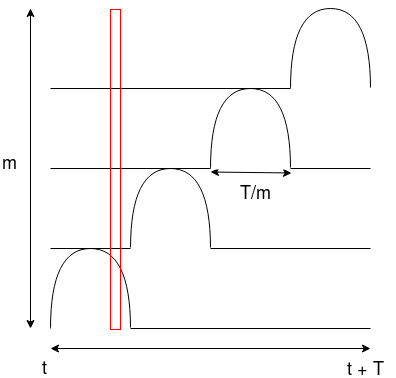
\includegraphics[width=0.4\textwidth]{images/HDTS_training}
\caption{Representation of the HDTS matrix. In the example the matrix $H$ has $m=4$ rows, which correspond to $m$ pulses of length $T/m$ milliseconds centred in the sub-interval $I_i$ for $i =1,\ldots,4$.
At each time step, a column of $H$ is selected (shown in red) and multiplied by a static weight matrix to construct the input current to the replay network.}
\label{fig:HDTS_training}
\end{figure}

\paragraph{HDTS usage}
The HDTS matrix $H$ is used to create an additional input to the reservoir during both the training and replay phase. For a correct functioning of the learning process, the timings of the presentation of the target signal and the HDTS input must completely overlap. Let $i \in [1, l]$ be the index that iterates through the target signal. At each time step, a column of the matrix $H$ is selected, $H_{:,i} \in \mathbb{R}^m$, and multiplied by the matrix $\eta_h \in \mathbb{R}^{N \times m}$, which components are uniformly drawned at random. The resulting  vector, $I_{HDTS} = \eta_h H_{:,i} \in \mathbb{R}^N$, is used as external input current to the reservoir.

\paragraph{HDTS pulses}
The HDTS can be constructed using several types of pulses. When learning multiple target signals, each signal should be coupled with a different pulse type. In this project a neural network is trained to learn four joint trajectories, so four pulse types were used. The four types of pulses are shown in \autoref{fig:HDTS_pulse_types}.

\begin{figure}[H]
\centering
\subfloat[upper sinusoid]{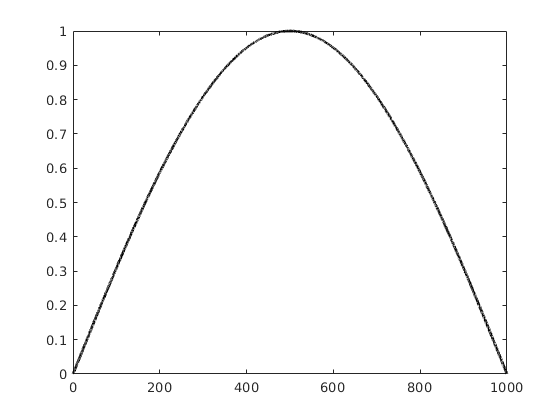
\includegraphics[width=0.25\columnwidth]{images/HDTS_pulse/hdts_upper_sinusoid.png} }
\subfloat[rectangular]{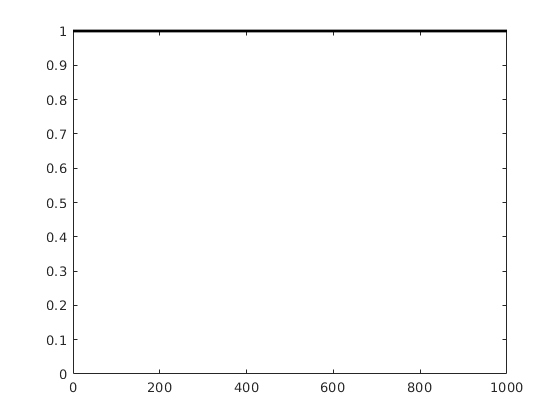
\includegraphics[width=0.25\columnwidth]{images/HDTS_pulse/hdts_rectangular.png} }
\subfloat[isosceles triangle]{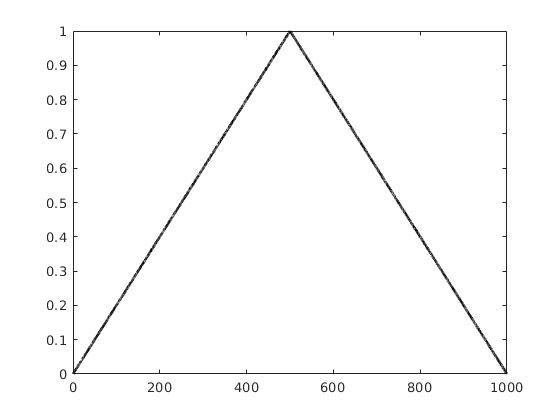
\includegraphics[width=0.25\columnwidth]{images/HDTS_pulse/hdts_isosceles_triangle.png} }
\subfloat[rectangular triangle]{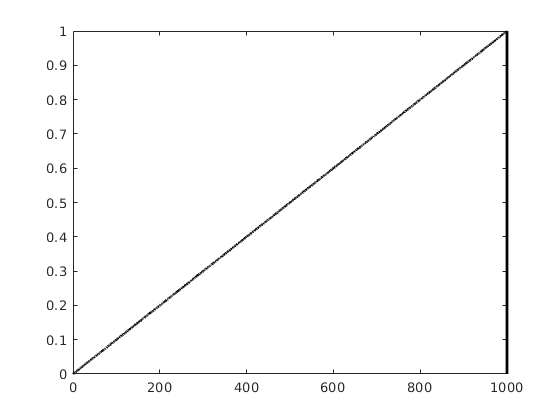
\includegraphics[width=0.25\columnwidth]{images/HDTS_pulse/hdts_rectangular_triangle.png} }
\caption{The four types of pulses used to construct the HDTS matrices. Each pulse has a maximum amplitude of 1.}
\label{fig:HDTS_pulse_types}
\end{figure}

More formally, the upper sinuosoid and the rectangular pulse types for the $i$-th row of $H$, can be respectively defined as in \eqref{eq:HDTS_sinuoid_pulse} and \eqref{eq:HDTS_rectangular_pulse} below

\begin{align}
H_{i,:} &= 
\begin{cases}
| \sin(\frac{\pi m t}{T}) | &, t \in I_i\\
0 &,  t \not \in I_i
\end{cases}\label{eq:HDTS_sinuoid_pulse}\\
H_{i,:} &= 
\begin{cases}
1 &,  t \in I_i\\
0 &, t \not \in I_i
\end{cases} \label{eq:HDTS_rectangular_pulse}
\end{align}

\paragraph{HTDS for accelerated replay}
Once the learning is finished, in order to replay the learned signal at different velocities, it is necessary to slightly modify the definitions of time sub-interval \eqref{eq:HDTS_interval} and HDTS \eqref{eq:HDTS_sinuoid_pulse}. A new factor $\rho > 0$ is introduced, that is used to compress or dilate time by multiplying the target signal length, obtaining $T \leftarrow T / \rho$. The new definitions of sub-interval \eqref{eq:HDTS_interval_rho} and HDTS pulse \eqref{eq:HDTS_pulse_rho} become as below

\begin{equation}
I_i = [\frac{T}{\rho} \cdot \frac{i-1}{m}, \frac{T}{\rho} \cdot \frac{i}{m}] \quad , i=1, \ldots, m
\label{eq:HDTS_interval_rho}
\end{equation}

\begin{equation}
H_{i,:} = 
\begin{cases}
| \sin(\frac{\pi m t}{T/ \rho}) | &, t \in I_i\\
0 &, otherwise
\end{cases}
\label{eq:HDTS_pulse_rho}
\end{equation}

In particular, with $\rho > 1$ the HDTS is compressed into a shorter time interval, while preserving the number of pulses $m$. As a result, each pulse is presented at a higher frequency and the network will replay the signal in accelerated velocity. Conversely with $\rho < 1$ the HDTS is dilated into a longer time interval. Each pulse has a lower frequency, and the target signal will be replayed at a slower pace.
An example of HDTS compression and dilation is shown in \autoref{fig:HDTS_rho}.

\begin{figure}[H]
\centering
\subfloat[$\rho = 1$\label{fig:HDTS_rho_1}]{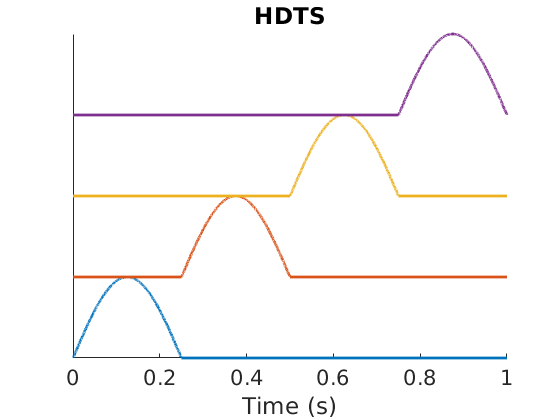
\includegraphics[width=0.3\textwidth]{images/HDTS_compression_per_1}}
\subfloat[$\rho = 0.5$\label{fig:HDTS_rho_0_5}]{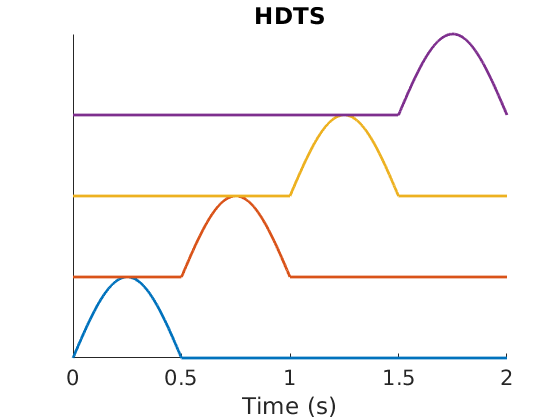
\includegraphics[width=0.3\textwidth]{images/HDTS_compression_per_0_5}}
\subfloat[$\rho = 2$\label{fig:HDTS_rho_2}]{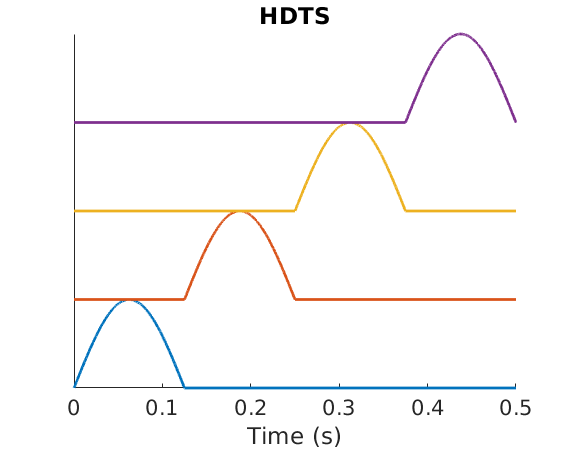
\includegraphics[width=0.3\textwidth]{images/HDTS_compression_per_2}}
\caption{Representation of an HDTS with $m=4$ pulses, and its compressed/dilated variants using compression factor $\rho$. \autoref{fig:HDTS_rho_1} With $\rho = 1$ it is obtained the original HDTS signal, which has length $T=1000$ milliseconds. \autoref{fig:HDTS_rho_0_5} Using $\rho = 0.5$ the HDTS is dilated into an interval of double length $T=2000$ milliseconds. \autoref{fig:HDTS_rho_2} Using $\rho = 2$ the HDTS is compressed into an interval of half length $T=500$.}
\label{fig:HDTS_rho}
\end{figure}

\paragraph{HTDS for inverse replay}
In order to replay the learned signal in inverse order, the columns of matrix $H$ should be flipped horizontally, to obtain a new matrix $H_{reverse}$ as illustrated below

\begin{equation}
H = 
\begin{bmatrix}
 H_{:,1} | H_{:,2} | \ldots | H_{:,l}
\end{bmatrix}
\Longrightarrow
H_{reverse} = 
\begin{bmatrix}
 H_{:,l} | H_{:,l-1} | \ldots | H_{:,1}
\end{bmatrix}
\end{equation}

\paragraph{HDTS for the interpolation/extrapolation of multiple signals}
Multiple HDTS signals can be used to learn multiple target functions. Post training it is possible to replay a signal by reinjecting the corresping HDTS pulses that were used during training, and switch to another activity by injecting a different pulse. 

Moreover, it is possible to linearly combine different HDTS pulse in order to create a new HDTS matrix that can be used as input during the replay phase.
Let $H_{(j)}$ be the HDTS matrix associated with trajectory $x_{(j)}$. A new HDTS matrix $H_{comb}$ is constructed as a linear combination of the known HDTS matrices 

\begin{equation}
H_{comb} = \sum_{j=1}^n \alpha_j H_{(j)}
\end{equation}

where $\alpha_j$ are the coefficients of the linear combination. In order to obtain an interpolation between the trajectories, it is necessary to use a convex combination, i.e. $\sum_{j=1}^n \alpha_j = 1$, otherwise any $\alpha$ coefficient can be used.




\chapter{Results}
\label{cap:result}
In the preliminary experiments it was choosen to use a family of sinusoidal waves as target signal with frequency $f$ Hz and phase $\varphi$. The reservoir had $N=2000$ neurons with $p=0.1$ connection probability.  

The simulation time $[t_0, t_{end}]$ is generally divided in three intervals. During $[t_0, t_{min}]$ the network stabilizes into a specific regime. The training takes place in during $(t_{min}, t_{crit})$ , where the readout weights are updated by means of RLS. The interval $[t_{crit}, t_{end})$ is used assess the quality of the learning scheme by measuring various metrics such as average firing rate and loss.

$G = 5 \times 10^3$, $Q \in \{0, 5 \times 10^3\}$. Integration time step $\delta t = 0.04$ ms.

The simulation performs $i_s = \lceil 1000 / \delta t \rceil$ iterations per second. Therefore the period of a target signal with frequency $f$ lasts $i_p = \lceil i_s / f \rceil$ iterations per period.

\section{Pre-training}
The first experiment consisted in performing a qualitative evaluation of the effect of applying an  external sinusoid to generate oscillations in the network activity. To this end it was played with the amplitude $A$ and the frequency $f$ of the oscillations. \autoref{fig:pre_learning_changing_A} shows a sample of 5 neurons membrane potential, the population activity and GNA variable for different values of $A \in \{0, 10, 50, 100, 200, 500 \}$ and fixed frequency $f=4 Hz$.  
The same information is shown in \autoref{fig:pre_learning_changing_f_osc} for a fixed amplitude $A=500$, varying the frequency $f \in \{4,7,10 \}$.

\paragraph{Discussion}
From \autoref{fig:pre_learning_changing_A} it can be seen that increasing $A$ corresponds to wider bursts, more evident synchronization, sharper GNA oscillations and higher slightly higher GNA values. In particular there were no oscillations generated with $A \in \{0, 10\}$. With $A=500$ there are perfectly synchronized, wide and clear bursts. However these could be entirely driven by the external signal given the high amplitude of the sinusoidal vawe. Instead with $A=200$ there could be more interesting hidden neuron interactions as the bursts are not as synchronized.

From \autoref{fig:pre_learning_changing_f_osc} it is clear to see that higher values of $f_{osc}$ correspond to more frequent oscillations per second, as expected.

% change A
\begin{figure}[H]
\centering
%\textbf{A=0}
\subfloat{\includegraphics[width=0.33\textwidth]{../Images/pre-learning/changing_A/membrane_A_0.png} }
\subfloat{\includegraphics[width=0.33\textwidth]{../Images/pre-learning/changing_A/raster_A_0.png} }
\subfloat{\includegraphics[width=0.33\textwidth]{../Images/pre-learning/changing_A/gna_A_0.png} }\\
%\textbf{A=10}
\subfloat{\includegraphics[width=0.33\textwidth]{../Images/pre-learning/changing_A/membrane_A_10.png} }
\subfloat{\includegraphics[width=0.33\textwidth]{../Images/pre-learning/changing_A/raster_A_10.png} }
\subfloat{\includegraphics[width=0.33\textwidth]{../Images/pre-learning/changing_A/gna_A_10.png} }\\
%\textbf{A=50}
\subfloat{\includegraphics[width=0.33\textwidth]{../Images/pre-learning/changing_A/membrane_A_50.png} }
\subfloat{\includegraphics[width=0.33\textwidth]{../Images/pre-learning/changing_A/raster_A_50.png} }
\subfloat{\includegraphics[width=0.33\textwidth]{../Images/pre-learning/changing_A/gna_A_50.png} }\\
%\textbf{A=100}
\subfloat{\includegraphics[width=0.33\textwidth]{../Images/pre-learning/changing_A/membrane_A_100.png} }
\subfloat{\includegraphics[width=0.33\textwidth]{../Images/pre-learning/changing_A/raster_A_100.png} }
\subfloat{\includegraphics[width=0.33\textwidth]{../Images/pre-learning/changing_A/gna_A_100.png} }\\
%\textbf{A=200}
\subfloat{\includegraphics[width=0.33\textwidth]{../Images/pre-learning/changing_A/membrane_A_200.png} }
\subfloat{\includegraphics[width=0.33\textwidth]{../Images/pre-learning/changing_A/raster_A_200.png} }
\subfloat{\includegraphics[width=0.33\textwidth]{../Images/pre-learning/changing_A/gna_A_200.png} }\\
%\textbf{A=500}
\subfloat{\includegraphics[width=0.33\textwidth]{../Images/pre-learning/changing_A/membrane_A_500.png} }
\subfloat{\includegraphics[width=0.33\textwidth]{../Images/pre-learning/changing_A/raster_A_500.png} }
\subfloat{\includegraphics[width=0.33\textwidth]{../Images/pre-learning/changing_A/gna_A_500.png} }\\
\caption{Pre-learning activity chaging amplitude of external oscillations, $A \in \{0, 10, 50, 100, 200, 500\}$.}
\label{fig:pre_learning_changing_A}
\end{figure}

% change f_osc
\begin{figure}[H]
\centering
\subfloat{\includegraphics[width=0.33\textwidth]{../Images/pre-learning/changing_f_osc/membrane_f_4.png} }
\subfloat{\includegraphics[width=0.33\textwidth]{../Images/pre-learning/changing_f_osc/raster_f_4.png} }
\subfloat{\includegraphics[width=0.33\textwidth]{../Images/pre-learning/changing_f_osc/gna_f_4.png} }\\
\subfloat{\includegraphics[width=0.33\textwidth]{../Images/pre-learning/changing_f_osc/membrane_f_7.png} }
\subfloat{\includegraphics[width=0.33\textwidth]{../Images/pre-learning/changing_f_osc/raster_f_7.png} }
\subfloat{\includegraphics[width=0.33\textwidth]{../Images/pre-learning/changing_f_osc/gna_f_7.png} }\\
\subfloat{\includegraphics[width=0.33\textwidth]{../Images/pre-learning/changing_f_osc/membrane_f_10.png} }
\subfloat{\includegraphics[width=0.33\textwidth]{../Images/pre-learning/changing_f_osc/raster_f_10.png} }
\subfloat{\includegraphics[width=0.33\textwidth]{../Images/pre-learning/changing_f_osc/gna_f_10.png} }\\
\caption{Pre-learning activity changing frequency of external oscillations $f \in \{4,7,10\}$ Hz.}
\label{fig:pre_learning_changing_f_osc}
\end{figure}


\section{Training}

We refer to \textit{continuous training} when the weight update is performed every $\Delta t = 20 \times \delta t = 0.8$ ms. We refer to \textit{phase training} when the weights are updated at a specific point of the phase of the target signal, only once per cycle.

\subsection{Changing the phase $\varphi_{sin}$ of the teaching signal}
Determine whether the phase of the teaching signal $\varphi_{sin} \in \{0 \pi, \frac{1}{2} \pi \}$ has an impact on the performance. The network is first stabilized for 5 seconds of simulation. The network is then trained for an amount of time corresponding to 20 cycles of the target signal. This choice was made to better compare the performance obtained with target signals of different frequencies $f \in \{0.3, 0.5, 0.8, 1, 5, 7, 12 \}$ Hz. The frequency of the external oscillations was fixed at $f = 4$ Hz, whereas it was varied the amplitude $A \in \{200, 500\}$. 

When FORCE training was turned off, the simulation was carried out for additional 10 target signal cycles. For each setting, it is computed the Average Firing Rate and the Average Squared Error between the target signal and the approximant, over the 10 post training cycles. Each result is obtained as the average of 10 repetitions. The Results are summarized in \autoref{tab:A_200_500}.

\paragraph{Discussion} Our approach performs slightly better than the Clopath settings for low frequency target signals. However for low-frequency target signals the Clopath settings perform considerably better. The pattern of best results do not depend on the phase of the target signal $\varphi_{sin}$.

% A = 200
% firing rate
\begin{table}[H]
\center
\caption{Comparison of Average Firing Rate and Average Error obtained by Our approach and the Clopath settings. The external sinuoid amplitude was $A \in \{200, 500\}$. The teaching signal phase was $\varphi_{sin} \in \{0 \pi, \frac{1}{2} \pi \}$. Training lasted for 20 cycles of the teaching signal. The results were averaged over 10 cycles after training, for 10 trials, plus/minus standard deviation shown. Best results shown in bold.}
\resizebox{\textwidth}{!}{%
\begin{tabular}{|c|ccc|ccc|}
\toprule
% sin phase = 0 pi
\bm{$\varphi_{sin} = 0 \pi$} & \multicolumn{3}{c|}{Average Firing Rate} & \multicolumn{3}{c|}{Average Error} \\ \hline
\multicolumn{1}{|c|}{$f_{sin}$} & $A=200$ & $A=500$ & Clopath  & $A=200$ & $A=500$ & Clopath  \\ \hline
\multicolumn{1}{|c|}{0.3} &  24.61 (1.17)  & 26.53 (0.67) & 29.00 (2.10)   &  \textbf{0.87 (0.12)}  & 0.91 (0.10) & 0.97 (0.17)   \\
\multicolumn{1}{|c|}{0.5} &  28.09 (1.11)  & 28.29 (0.80) & 29.78 (0.62)  &  1.06 (0.14)  & \textbf{0.83 (0.10)}  & 0.99 (0.21)   \\
\multicolumn{1}{|c|}{0.8} &  27.48 (0.99)  & 27.87 (0.84) & 28.27 (0.90)  &  0.98 (0.25)  & \textbf{0.82 (0.22)} & 0.84 (0.47)  \\
\multicolumn{1}{|c|}{1}   &  27.62 (0.93)  & 28.71 (0.69) & 28.81 (0.97)  &  \textbf{0.26 (0.35)}  & 0.31 (0.38) & 0.66 (0.54)   \\
\multicolumn{1}{|c|}{5}   &  27.39 (1.46)  & 26.93(1.92) & 36.52 (0.85)   &  0.50 (0.34)  & 0.71 (0.27) &\textbf{0.05 (0.03)}    \\
\multicolumn{1}{|c|}{7}   &  29.96 (1.83)  & 26.92 (1.15) & 36.64 (1.00)   &  0.48 (0.23)  & 0.64 (0.14)  & \textbf{0.05 (0.04)}    \\
\multicolumn{1}{|c|}{12}  &  25.50 (3.03)  & 21.46 (1.42) & 37.33 (0.67)   &  0.32 (0.15)  & 0.29 (0.06)  & \textbf{0.02 (0.02)}    \\
\bottomrule

\multicolumn{7}{c}{}\\
% sin phase = 0.5 pi
\toprule
\bm{$\varphi_{sin} = \frac{1}{2} \pi$} & \multicolumn{3}{c|}{Average Firing Rate} & \multicolumn{3}{c|}{Average Error} \\ \hline
\multicolumn{1}{|c|}{$f_{sin}$} & $A=200$ & $A=500$ & Clopath   & $A=200$  &  $A=500$ & Clopath  \\ \hline
\multicolumn{1}{|c|}{0.3} &  24.31 (0.84) & 26.45 (0.96) & 28.63 (1.41)  &  \textbf{0.86 (0.12) }  & 0.91 (0.11) & 0.94 (0.12)       \\
\multicolumn{1}{|c|}{0.5} & 27.48 (1.30)  & 28.11 (0.79) & 29.08 (1.04)  & 1.02 (0.13)   & \textbf{0.90 (0.13)} &	0.93 (0.11)	\\
\multicolumn{1}{|c|}{0.8} & 26.66 (1.30)  & 28.77 (1.12) & 28.01 (1.09)  & 0.99 (0.15)   & \textbf{0.93 (0.38)}  & 1.03 (0.25)        \\
\multicolumn{1}{|c|}{1}   & 27.82 (0.66)  & 29.18 (0.65) & 28.36 (0.89)  & \textbf{0.28 (0.36)}   & 0.68 (0.62) & 	0.53 (0.42)	\\
\multicolumn{1}{|c|}{5}   & 28.67 (0.85)  & 26.22 (1.39) & 37.12 (0.74)  & 0.66 (0.39)  & 0.76 (0.28)  &  \textbf{0.02 (0.03)}         \\
\multicolumn{1}{|c|}{7}   & 30.64 (2.34)  & 26.34 (2.14) & 37.62 (0.71)  & 0.60 (0.36)   & 0.64 (0.17)  & \textbf{0.02 (0.02)}      \\
\multicolumn{1}{|c|}{12}  & 25.84 (2.07) & 22.61 (0.90) & 37.81 (0.82)  &  0.38 (0.16) & 0.26 (0.01) & \textbf{0.01 (0.00)}     \\ \bottomrule
\end{tabular}
}
\label{tab:A_200_500}
\end{table}

\subsection{"Computing derivatives"}
The standard Clopath settings were modified in order to make the network to learn to approximate first order derivatives with respect to an arbitrary period $t_{past} < t$.

The simulation interval $[t_{crit}, t_{end}]$ was split in two sub-intervals, or stages: $[t_{crit}, t_{crit_2})$ and $[t_{crit_2}, t_{end}]$. In addition, during the interval $(t_0, t_{crit_2})$ a smoothed version of the original target signal was injected as input current (see \eqref{eq:current_past} below).

Let $A \in \mathbb{R}$ be the amplitude of the injected target signal, and $p$ be the percentage of neurons that receive the additional current. The binary vector $I_{TR} \in \{0,1\}^N$ represents the input target recipients, where each entry is 1 with probability $p$ and 0 otherwise.  
Let $I_{TIC} \in \mathbb{R}^N$ be the input target indiv. coefficient, where each entry is drawn from a gaussian distribution, $\mathcal{N}(\mu, \sigma)$, with mean $\mu$ and standard deviation $\sigma$. 
The input target coefficient $I_{TC} \in \mathbb{R}^N$ that is injected as current is defined as

\begin{equation}
I_{TC} = A \cdot I_{TR} \odot I_{TIC}
\label{eq:input_target_coefficient}
\end{equation}

where $\odot$ is the component-wise product. The term \eqref{eq:input_target_coefficient} is used to augment the input current as below

\begin{equation}
I = 
\begin{cases} 
IPSC + \eta \hat{x}(t- \delta_t) + BIAS + x(t) \odot I_{TC} &,\qquad t \in (t_0, t_{crit_2}) \\
IPSC + \eta \hat{x}(t- \delta_t) + BIAS &,\qquad otherwise
\end{cases}
\label{eq:current_past}
\end{equation}

The average error was computed both for the stages $[t_{crit}, t_{crit_2})$ and $[t_{crit_2}, t_{end}]$, as well as across the entire post-training interval $[t_{crit}, t_{end}]$, with respect to previous observations of the target signal as

\begin{equation}
e = \hat{x}(t) - x(t - t_{past})
\end{equation}

The training settings are as follows. 
$t_{min} = 3$ seconds, $t_{crit} = t_{min} + \max \{5 s, 20 \cdot i_p \}$, where $i_p$ is the number of simulation iterations per period.
$t_{crit_2} = t_{crit} + \max \{ 5 s, 10 \cdot i_p \}$,
$t_{end} = t_{crit_2} + \max \{8 s, 10 \cdot i_p \}$. $A = 30$, $p=0.2$. $\mu = 0.5$, $\sigma = 0.5$.

The results are shown in \autoref{fig:past} for $t_{past} \in [0, 100]$ ms and target signal frequency $f \in \{ 1,5,7,12 \}$.

%Feedback term: 0, 5000

\begin{figure}[H]
\centering
\subfloat[$f = 1$ Hz]{\includegraphics[width=0.5\textwidth]{../Images/learning/past/past_f_1_Q_5000.png}}
\subfloat[$f = 5$ Hz]{\includegraphics[width=0.5\textwidth]{../Images/learning/past/past_f_5_Q_5000.png}}\\
%\subfloat[$Q = 0$]{\includegraphics[width=0.5\textwidth]{../Images/learning/past/past_f_5_Q_0.png}}\\
\subfloat[$f = 7$ Hz]{\includegraphics[width=0.5\textwidth]{../Images/learning/past/past_f_7_Q_5000.png}}
\subfloat[$f = 12$ Hz]{\includegraphics[width=0.5\textwidth]{../Images/learning/past/past_f_12_Q_5000.png}}\\
\caption{Squared error vs $t_{past} \in [0,100]$ computed across the entire post-training period $[t_{crit}, t_{end}]$, stage one $[t_{crit}, t_{crit_2})$, and stage two $[t_{crit_2}, t_{end}]$. Target signal frequency $f \in \{1, 5, 7, 12\}$.}
\label{fig:past}
\end{figure}

\subsection{Discretization of the target signal}
Starting from the standard Clopath settings, it was experimented with target discretization and smoothing.
%CLOPATH settings (continuous 5-10-15 training)
Let $x(t) \in \mathbb{R}$ be the original unidimensional target signal. 
Let $x_{01}(t) \in \{0,1\}^m$ be the one-hot representation of the target signal after its discretization into $m$ uniform bins \footnote{The target discretization was achieved by means of the Matlab \textit{discretize()} built-in function.}. Each bin $b_i$, for $i=1, \ldots, m$, accounts for a certain contiguous subset of the target signal codomain, entirely defined by the interval $[b_i^L, b_i^H]$, which correspond to the lower and upper extreams of the signal values for that bin.
Let $x_s(t) \in \mathbb{R}^m$ be a smoothed version of the one-hot encoded target obtained after the application of a gaussian filter.

% e_i base canonica

%First the target signal $x(t)$ is discretized into $m$ uniform bins \footnote{The target discretization was achieved by means of the Matlab \textit{discretize()} built-in function.}. The bins are then one-hot encoded to obtain an m-dimensional signal $x_{01}(t) \in \{0,1\}^m$. Then the following strategies have been tested independently.

\paragraph{One-hot input, continuous m-dimensional output (WRONG)}
The network takes as input an m-dimensional one-hot encoded signal $x_{01}(t) \in \{0,1\}^m$ and outputs an m-dimensional continuous vector $\hat{x}(t) \in \mathbb{R}^m$. The loss is computed the sum of squared errors: $\mathcal{L}(t) = \sum_{i=1}^m (x_{01_i}(t) - \hat{x}_i(t))^2$. (see \autoref{tab:one_hot_target_continuous_output})

% metti tabella
% One-hot input, continuous m-dimensional continuous output
\begin{table}[H]
\centering
\begin{tabular}{c|c|c|}
\cline{2-3}
                          & \multicolumn{2}{|c|}{$m= 10$}            \\ \hline
\multicolumn{1}{|c|}{$f_{sin}$} & Average Firing Rate & Average Error     \\ \hline
\multicolumn{1}{|c|}{0.3} & 48.02 (3.26)  & 2.46 (0.34) \\
\multicolumn{1}{|c|}{0.5} & 46.16 (3.73)  & 2.15 (0.29) \\
\multicolumn{1}{|c|}{0.8} & 42.72 (4.09)  & 1.74 (0.24) \\
\multicolumn{1}{|c|}{1}   & 40.53 (3.82)  & 1.58 (0.28) \\
\multicolumn{1}{|c|}{5}   & 40.88 (1.80)  & 1.29 (0.20) \\
\multicolumn{1}{|c|}{7}   & 38.38 (3.29)  & 1.36 (0.13) \\
\multicolumn{1}{|c|}{12}  & 23.31 (1.69)  & 1.05 (0.04) \\ \hline
\end{tabular}
\caption{Target discretization, $m=10$ bins. One-hot input, continuous m-dimensional continuous output}
\label{tab:one_hot_target_continuous_output}
\end{table}

\paragraph{One-hot input, one hot target, multi-class misclassification error}
The network takes as input the one-hot encoded signal $x_{01}(t) \in \mathbb{R}^m$ and outputs an m-dimensional continuous vector $\hat{x}(t) \in \mathbb{R}^m$. 
The prediction is then converted to a one-hot vector, $\hat{x}(t) \rightarrow \hat{x}_{01}(t) \in \{0,1\}^m$. 
The loss is computed as the misclassification error: $\mathcal{L}(t) =  \mathbf{1}(x_{01}(t)== \hat{x}_{01}(t))$, where $\mathbf{1}(\cdot)$ is the indicator function. (see \autoref{tab:one_hot_target_one_hot_output})

% metti tabella
%one-hot input, one hot target - multi-class misclassification error
\begin{table}[H]
\centering
\begin{tabular}{c|c|c|}
\cline{2-3}
                          & \multicolumn{2}{|c|}{$m= 10$}            \\ \hline
\multicolumn{1}{|c|}{$f_{sin}$} & Average Firing Rate & Average misclassification Error     \\ \hline
\multicolumn{1}{|c|}{0.3} & 46.07 (3.21)  & 0.93 (0.03) \\
\multicolumn{1}{|c|}{0.5} & 44.05 (9.05)  & 0.86 (0.04) \\
\multicolumn{1}{|c|}{0.8} & 41.89 (4.40)  & 0.87 (0.03) \\
\multicolumn{1}{|c|}{1}   & 38.61 (2.05)  & 0.90 (0.03) \\
\multicolumn{1}{|c|}{5}   & 40.63 (1.93)  & 0.76 (0.19) \\
\multicolumn{1}{|c|}{7}   & 38.43 (1.90)  & 0.88 (0.05) \\
\multicolumn{1}{|c|}{12}  & 22.54 (0.71)  &  0.92 (0.02)\\ \hline
\end{tabular}
\caption{Target discretization, $m=10$ bins. One-hot input, one hot target - multi-class misclassification error}
\label{tab:one_hot_target_one_hot_output}
\end{table}

\paragraph{One-hot input, maxout target}
It was tried to reconstruct the monodimensional target $x(t)$ from the $m$ readouts.
The network takes as input the one-hot encoded signal $x_{01}(t) \in \mathbb{R}^m$ and outputs an m-dimensional continuous vector $\hat{x}(t) \in \mathbb{R}^m$. The loss is computed as the squared error between the original target and the maximum of the readouts: $\mathcal{L}(t) =  (x(t) - \max_i \hat{x}_i(t))^2$. (see \autoref{tab:one_hot_input_maxout_target})

% metti tabella
% one-hot input, maxout target
\begin{table}[H]
\centering
\begin{tabular}{c|c|c|}
\cline{2-3}
                          & \multicolumn{2}{|c|}{$m= 10$}            	\\ \hline
\multicolumn{1}{|c|}{$f_{sin}$} & Average Firing Rate & Average Error    \\ \hline
\multicolumn{1}{|c|}{0.3} & 46.07 (3.21)  & 1.46 (0.31) \\
\multicolumn{1}{|c|}{0.5} & 44.05 (9.05)  & 1.45 (0.39) \\
\multicolumn{1}{|c|}{0.8} & 41.89 (4.40)  & 1.26 (0.33) \\
\multicolumn{1}{|c|}{1}   & 38.61 (2.05)  & 0.92 (0.09) \\
\multicolumn{1}{|c|}{5}   & 40.59 (1.87)  & 1.07 (0.06) \\
\multicolumn{1}{|c|}{7}   & 38.43 (1.90)  & 1.03 (0.08) \\
\multicolumn{1}{|c|}{12}  & 22.54 (0.71) & 0.60 (0.01) \\ \hline
\end{tabular}
\caption{Target discretization, $m=10$ bins. One-hot input, one hot target - max-out}
\label{tab:one_hot_input_maxout_target}
\end{table}

\paragraph{One-hot + smoothing input, maxout target}
The network takes as input a smoothed version of the one-hot encoded signal $x_{01}(t) \in \mathbb{R}^m$, which is constructed as follows.
Let $x_0 = [\mu_1, \ldots, \mu_m ]^\intercal$ be the vector of bin centres, where $\mu_i = \frac{b_i^L + b_i^R}{2}.$
It is constructed an m-dimensional vector $\vec{x}(t)$ which elements are $m$ replicas of the value of the monodimensional target signal $x(t)$, $\vec{x}(t) = [x(t), \ldots, x(t)]^\intercal \in \mathbb{R}^m$.
Then the smoothed m-dimensional target signal $x_s(t)$ is constructed by applying a gaussian kernel of the form:

\begin{equation}
x_s(t) = e^{-\frac{(\vec{x}(t) - x_0)^2}{\sigma_s}}\qquad\forall t
\end{equation}

where $\sigma_s$ is the standard deviation of the smoothing kernel. The network outputs an m-dimensional continuous vector $\hat{x}_s(t) \in \mathbb{R}^m$.
The loss is computed as the squared error between the maximum of the readouts and the original target signal: $\mathcal{L}(t) =  (x(t) - \max_i \hat{x}_{s_i}(t))^2$. (see \autoref{tab:one_hot_smoothed_input_maxout_target_sigma_1} and \autoref{tab:one_hot_smoothed_input_maxout_target_sigma_0_001})

% metti tabella
%one-hot + smoothing input (sigma=1), maxout target
\begin{table}[H]
\centering
\begin{tabular}{c|c|c|}
\cline{2-3}
                          & \multicolumn{2}{|c|}{$m= 10$}            \\ \hline
\multicolumn{1}{|c|}{$f_{sin}$} & Average Firing Rate & Average Error     \\ \hline
\multicolumn{1}{|c|}{0.3} & 150.24 (62.55) & 55.37 (67.87) \\
\multicolumn{1}{|c|}{0.5} & 37.93 (30.34)  &  1.51 (1.16) \\
\multicolumn{1}{|c|}{0.8} & 17.34 (8.53)  & 0.71 (0.18) \\
\multicolumn{1}{|c|}{1}   & 38.55 (24.00)  & 1.03 (0.36) \\
\multicolumn{1}{|c|}{5}   &  80.56 (1.62) & 1.49 (0.01) \\
\multicolumn{1}{|c|}{7}   &  80.62 (1.70) & 1.49 (0.01) \\
\multicolumn{1}{|c|}{12}  &  77.46 (8.52) & 1.43 (0.17) \\ \hline
\end{tabular}
\caption{Target discretization, $m=10$ bins. one-hot + smoothing input ($\sigma_s = 1$), maxout target}
\label{tab:one_hot_smoothed_input_maxout_target_sigma_1}
\end{table}

%one-hot + smoothing input (sigma=0.001), maxout target
\begin{table}[H]
\centering
\begin{tabular}{c|c|c|}
\cline{2-3}
                          & \multicolumn{2}{|c|}{$m= 10$}            \\ \hline
\multicolumn{1}{|c|}{$f_{sin}$} & Average Firing Rate & Average Error     \\ \hline
\multicolumn{1}{|c|}{0.3} & 19.95 (3.49) & 0.56 (0.19)\\
\multicolumn{1}{|c|}{0.5} & 17.75 (9.50)  & 0.55 (0.04)  \\
\multicolumn{1}{|c|}{0.8} & 1.95 (6.18)  & 0.51 (0.03) \\
\multicolumn{1}{|c|}{1}   & 10.64 (9.19)  & 0.53 (0.03) \\
\multicolumn{1}{|c|}{5}   & 12.31 (0.19)  & 0.51 (0.00) \\
\multicolumn{1}{|c|}{7}   & 11.46 (0.28)  & 0.51 (0.00) \\
\multicolumn{1}{|c|}{12}  & 11.02 (0.52) & 0.51 (0.00) \\ \hline
\end{tabular}
\caption{Target discretization, $m=10$ bins. one-hot + smoothing input ($\sigma_s = 0.001$), maxout target}
\label{tab:one_hot_smoothed_input_maxout_target_sigma_0_001}
\end{table}

\paragraph{One-hot + smoothing input, maxout target, selective feedback}
The experiment described in the previous paragraph is augmented by modifying the feedback term of the FORCE training. In the Clopath settings, at each time step $t$ a feedback term is reinjected as input current, defined as $\eta \hat{x}_s(t-\delta t) \in \mathbb{R}^N$. In this experiment the feedback term was modified by substituting the matrix $\eta$ with $\eta'$, so that each dimension of the output $\hat{x}_s(t-\delta t)$ is reinjected only to a subset of $N/m$ neurons. In this way different neurons will learn to fire when the signal belongs to different bins. \autoref{fig:selective_feedback} illustrates the procedure for creating the matrix $\eta'$.

\begin{equation}
\eta \hat{x}_s = 
\left[
\begin{array}{cccc}
* & * & * \\
* & * & * \\
* & * & * \\
* & * & * \\
* & * & * \\
* & * & * \\
\end{array}
\right]
\begin{bmatrix}
           \hat{x}_{s_1} \\
           \hat{x}_{s_2} \\
           \hat{x}_{s_3}
\end{bmatrix}
\longrightarrow
\eta' \hat{x}_s = 
\left[
\begin{array}{cccc}
* & 0 & 0 \\
* & 0 & 0\\
\hline
0 & * & 0\\
0 & * & 0\\
\hline
0 & 0 & * \\
0 & 0 & * \\
\end{array}
\right]
\begin{bmatrix}
           \hat{x}_{s_1} \\
           \hat{x}_{s_2} \\
           \hat{x}_{s_3}
\end{bmatrix}        \nonumber
\end{equation}
\captionof{figure}{Example of the construction of the selective feedback matrix $\eta'$ from $\eta$, using $N = 6$ neurons and $m=3$ bins. The rows of matrix $\eta'$ are virtually divided in $m$ blocks. In the $i$-th block, all the values are set to 0 except for the $i$-th row subset, so that each dimension $\hat{x}_{s_i}$ only influences one cluster of neurons.}
\label{fig:selective_feedback}

\todo{do some experiments, simple data manipulation}

\begin{figure}[H]
\centering
\subfloat[]{\includegraphics[width=0.5\textwidth]{../Images/learning/multidim_target/discretized_signal.png} }
\subfloat[]{\includegraphics[width=0.5\textwidth]{../Images/learning/multidim_target/bin_histogram.png} }\\
\subfloat[$\sigma=1$]{\includegraphics[width=0.5\textwidth]{../Images/learning/multidim_target/smoothed_dimensions_sigma_1.png} }
\subfloat[$\sigma=0.05$]{\includegraphics[width=0.5\textwidth]{../Images/learning/multidim_target/smoothed_dimensions_sigma_0_05.png} }
\caption{Example of target discretization in $m=5$ bins. An $m$-dimensional one-hot encoded target signal is created and then smoothed with gaussian pulses centred at in the middle of each sub-interval. For a given sample, the value in each dimension represents the membership value to a particular bin. The standard deviation $\sigma$ of the gaussians determine how much the intervals overlap.}
\label{fig:target_discretization_example}
\end{figure}

%% change d to control frequency

\section{Control the replay velocity changing the spike frequency adaption}
Original Clopath settings, change $d \in \{-50, 0, 50, 100, 150, 200 \}$.
See \autoref{fig:error_and_firing_rate_vs_d}.

\begin{figure}[H]
\centering
\subfloat[]{\includegraphics[width=0.5\textwidth]{../Images/learning/try_to_make_low_frequency_work/average_error_vs_d.png} }
\subfloat[]{\includegraphics[width=0.5\textwidth]{../Images/learning/try_to_make_low_frequency_work/average_firing_rate_vs_d.png} }\\
\caption{Average squared error and average firing rate as a function of parameter $d \in \{-50, 0, 50, 100, 150, 200 \}$, for target sinusoids of frequency $f \in \{0.3, 0.5, 0.8, 1, 5, 7, 12 \}$.}
\label{fig:error_and_firing_rate_vs_d}
\end{figure}

\todo{put raster plots, voltage and recovery traces, and maybe phase portraits with d=-50, d=0, d= 50/200}


\todo{describe in a more abstract way}
$N = 100$ because it is faster and qualitatively you get the same results,
$f = 1$ Hz,
$\delta_t = 0.2$ so it is faster,
start with $d = -50$ then change it every 10 seconds post-learning during the interval $[t_{crit}, t_{end}]$
every 10 seconds change parameter,
$t_{min} = 3$ seconds, $t_{crit} = 10$ seconds, $t_{crit_2} = 15$ seconds, $t_{end} = 135$ seconds. 
(i.e 2 minutes of parameter change)
\todo{does the network still start in a chaotic regime when using d=0 or negative?}


In \autoref{fig:change_d_control_frequency} are shown the target approximant and spectrogram for three cases: 
\autoref{fig:d_increased} $d \leftarrow d + 20$ for 2 minutes,
\autoref{fig:d_decreased} $d \leftarrow d - 5$ for 2 minutes,
\autoref{fig:d_icr_decr}  $d \leftarrow d + 20$ for the fist minute and $d \leftarrow d - 20$ in the second minute.

In \autoref{fig:change_d_control_frequency}
\autoref{fig:a_increased} $a \leftarrow a + 0.005$ for 2 minutes,
\autoref{fig:a_decreased} $a \leftarrow a - 0.00025$ for 2 minutes,
\autoref{fig:a_icr_decr}  $a \leftarrow a + 0.005$ for the fist minute and $a \leftarrow a - 0.005$ in the second minute.

% change d
\begin{figure}[H]
\centering
\subfloat[\label{fig:d_increased}]{\includegraphics[width=0.33\textwidth]{../Images/learning/try_to_make_low_frequency_work/control_frequency/approximant_d_plus_20.png}}
\subfloat[\label{fig:d_decreased}]{\includegraphics[width=0.33\textwidth]{../Images/learning/try_to_make_low_frequency_work/control_frequency/approximant_d_minus_5.png}}
\subfloat[\label{fig:d_icr_decr}]{\includegraphics[width=0.33\textwidth]{../Images/learning/try_to_make_low_frequency_work/control_frequency/approximant_d_plus_20_minus_20.png}}\\

\subfloat[]{\includegraphics[width=0.33\textwidth]{../Images/learning/try_to_make_low_frequency_work/control_frequency/spectrogram_d_plus_20.png}}
\subfloat[]{\includegraphics[width=0.33\textwidth]{../Images/learning/try_to_make_low_frequency_work/control_frequency/spectrogram_d_minus_5.png}}
\subfloat[]{\includegraphics[width=0.33\textwidth]{../Images/learning/try_to_make_low_frequency_work/control_frequency/spectrogram_d_plus_20_minus_20.png}}

\caption{Changing the spiking frequency adaptation (parameter $d$) post training. The network is set onto a chaotic attractor during the first 5 seconds of simulation (first white region). Training takes place for 5 seconds (gray region). Post training, the network reproduces the learned signal for additional 5 seconds (second white region). The parameter $d$ is linearly changed every 10 seconds for 2 minutes (red region): \autoref{fig:d_increased} $d$ increased; \autoref{fig:d_decreased} $d$ decreased; \autoref{fig:d_icr_decr} $d$ increased then decreased.}
\label{fig:change_d_control_frequency}
\end{figure}

% change a
\begin{figure}[H]
\centering
\subfloat[\label{fig:a_increased}]{\includegraphics[width=0.33\textwidth]{../Images/learning/try_to_make_low_frequency_work/control_frequency/approximant_a_plus_0_005.png}}
\subfloat[\label{fig:a_decreased}]{\includegraphics[width=0.33\textwidth]{../Images/learning/try_to_make_low_frequency_work/control_frequency/approximant_a_minus_0_00025.png}}
\subfloat[\label{fig:a_icr_decr}]{\includegraphics[width=0.33\textwidth]{../Images/learning/try_to_make_low_frequency_work/control_frequency/approximant_a_plus_0_005_minus_0_005.png}}\\

\subfloat[]{\includegraphics[width=0.33\textwidth]{../Images/learning/try_to_make_low_frequency_work/control_frequency/spectrogram_a_plus_0_005.png}}
\subfloat[]{\includegraphics[width=0.33\textwidth]{../Images/learning/try_to_make_low_frequency_work/control_frequency/spectrogram_a_minus_0_00025.png}}
\subfloat[]{\includegraphics[width=0.33\textwidth]{../Images/learning/try_to_make_low_frequency_work/control_frequency/spectrogram_a_plus_0_005_minus_0_005.png}}

\caption{Changing the spiking frequency adaptation (parameter $a$) post training. The network is set onto a chaotic attractor during the first 5 seconds of simulation (first white region). Training takes place for 5 seconds (gray region). Post training, the network reproduces the learned signal for additional 5 seconds (second white region). The parameter $a$ is linearly changed every 10 seconds for 2 minutes (red region): \autoref{fig:a_increased} $a$ increased; \autoref{fig:a_decreased} $a$ decreased; \autoref{fig:a_icr_decr} $a$ increased then decreased.}
\label{fig:change_a_control_frequency}
\end{figure}

\section{Using high-dimensional temporal signals}
\label{sec:HDTS_synthetic_datasets}
This section reports the results of the experiments performed on the synthetic datasets, with the goal of getting familiar with using the HDTS techniques discussed in \autoref{sec:HDTS}, uncovering their potential and observing possible limitations.

\subsection{HDTS speeds up the replay}
To verify that the compression and dilation of the HDTS correctly accelerates and decelerates the replay phase, the network was trained to learn one period of a sinuoid. The choice of this supervisor was made because it is clear to observe the change of the replay frequency from the spectrogram of the network output. Post training the network successfully replayed the signal. After few repetitions, the HDTS was first compressed then dilated, resulting in a correct acceleration and deceleration of the signal replay, see \autoref{fig:HDTS_speedup_replay}. 

\begin{figure}[H]
\centering
$\bm{\rho=2}$
\subfloat{\includegraphics[width=0.5\textwidth]{../Images/learning/HDTS/speedup/target_vs_approx_supervisor_2_compress_2.png} }
\subfloat{\includegraphics[width=0.5\textwidth]{../Images/learning/HDTS/speedup/spectro_supervisor_2_compress_2.png} }\\
$\bm{\rho=0.5}$
\subfloat{\includegraphics[width=0.5\textwidth]{../Images/learning/HDTS/speedup/target_vs_approx_supervisor_2_compress_0_5.png} }
\subfloat{\includegraphics[width=0.5\textwidth]{../Images/learning/HDTS/speedup/spectro_supervisor_2_compress_0_5.png} }
\caption{Acceleration ($\rho=2$) and deceleration ($\rho=0.5$) of the replay of a sinuoid with original frequency $1 Hz$. Despite the noise and amplitude errors, the network properly adjusts the velocity of the replay. The original signal is shown with a black line also during the acceleration/deceleration phase, to better see the difference with the network output.}
\label{fig:HDTS_speedup_replay}
\end{figure}

The trend of the network output visibly resembles the target signal, although it presents some high-frequency oscillations. This does not constitute a major limitation, because the high-frequency oscillations could be removed applying a low-pass filter. The output also presents a marginal amplitude error. The same behavior was also verified with non-periodic target signals (not shown).

\subsection{Inverse replay}
It was verified that the FORCE method combined with HDTS allows the inverse replay of a signal. This could be useful for a robotic arm that wants to perform an activity in a certain position and then go back to the original position. 

It was trained a network for three repetitions of the signal. Post training the network replayed the learned signal for one repetition. After that, it was injected the reversed version of the HDTS, $H_{reverse}$. As is shown in \autoref{fig:HDTS_inverse}, the network inverted the replay successfully, although with some loss in accuracy as reported in \cite{nicola2017supervised}.

\todo{redo picture with colored icrit2 part}

\begin{figure}[H]
\centering
\subfloat{\includegraphics[width=0.5\textwidth]{../Images/learning/HDTS/inverse/target_vs_approx_sup1.png} }
\subfloat{\includegraphics[width=0.5\textwidth]{../Images/learning/HDTS/inverse/target_vs_approx_sup2.png} }
\caption{The inverse application of the HDTS makes the network replay the signal backwards.}
\label{fig:HDTS_inverse}
\end{figure}

\subsection{HDTS triggers the replay}
For the purpose of this project, it was interesting to asses whether it is possible to trigger the replay of the target signal by turning on/off the HDTS when desired. In order to obtain this effect, the HDTS was turned turned off for 2 seconds post training. As a result the network immediately stopped the replay of the target signal. When the HDTS was reinjected again, the network successfully restarted the replay, see \autoref{fig:HDTS_triggers}. The experiment was performed for two supervisors.
\todo{if you set BIAS=0 when HDTS=0 the network stops spiking.}

% HDTS trigger the replay
\begin{figure}[H]
\centering
\subfloat[dataset 1]{\includegraphics[width=0.5\textwidth]{../Images/learning/HDTS/does_it_trigger/target_vs_approx_2.png} }
\subfloat[dataset 3]{\includegraphics[width=0.5\textwidth]{../Images/learning/HDTS/does_it_trigger/target_vs_approx_1.png} }
\caption{HDTS triggers the replay of the signal. At 6 seconds the HDTS is removed and the network immediately stops reproducing the signal. The HDTS is reinjected after 2 seconds triggering the immediate replay of the singal.}
\label{fig:HDTS_triggers}
\end{figure}

\subsection{Multiple HDTS to learn multiple signals}
In the previous section it was shown that turning on and off the injection of the HDTS triggers the replay of the target signal. The next question to answer was whether it is possible to use multiple HDTS to learn multiple outputs, and make the network switch between activities when desired. The experiment was done for two supervisors, hence two different HDTS pulse types were used (positive sinusoid and rectangular pulse) and combined into an HDTS train, see Figure \autoref{fig:HDTS_train}. During training the two supervisors were presented to the network a couple of times intermittently, along with the corresponding HDTS pulse type. Post training both the HDTS were removed, and then reinjected separately at different times to make the network replay the different target signals, see Figure \autoref{fig:approx_vs_target_two_target_two_HDTS}. The network successfully learned the two signals as a function of the two HDTS and was able to repeat them when triggered with the proper HDTS. However the network output presented a strange upward excursion when the second HDTS was turned off. Changing the order in which the HDTS were proposed or using different pulse types resulted in analogous behaviours.

It was also wondered what would happen using only one HDTS pulse type to learn two different signals. It was speculated that the network could remember the last signal presented during training.
But as expected, using the same type of HDTS to learn two different signals completely destroyed the learning process, see \autoref{fig:one_HDTS_two_targets}.

\todo{If you set BIAS=0 when HDTS=0 the network does not completely stop spiking.}

% multiple HDTS to learn multiple target signals
\begin{figure}[H]
\subfloat[\label{fig:HDTS_train}]{\includegraphics[width=1\textwidth]{images/HDTS_train.png}}\\
\subfloat[\label{fig:approx_vs_target_two_target_two_HDTS}]{\includegraphics[width=0.5\textwidth]{../Images/learning/HDTS/approx_vs_target_two_target_two_HDTS.png} }
\subfloat[]{\includegraphics[width=0.5\textwidth]{../Images/learning/HDTS/raster_two_target_two_HDTS.png}}
\caption{Learning two different target signals. \autoref{fig:HDTS_train} Example of HDTS train using sinusoidal and rectangular pulses to learn two different objective signals. Flat line segments indicate the absence of HDTS. Post training, changing the type of HDTS the network changes activity replaying a different signal. The removal of the HDTS at time 5 seconds and 10 seconds results in a strange excursion of the network output. }
\label{fig:multi_HDTS_multi_target} 
\end{figure}

\begin{figure}[H]
\centering
\subfloat{\includegraphics[width=0.5\textwidth]{../Images/learning/HDTS/one_HDTS_two_targets_destroy.png}} 
\caption{Using only one HDTS pulse type to learn two different signals completely destroys the learning process. For convenience, the target signal is shown as a flat black line post training.}
\label{fig:one_HDTS_two_targets}
\end{figure}

\todo{not clear what happens when we remove the HDTS.}
\todo{how to define rest? keep robot in a steady position, no spikes?}

\subsection{Signal interpolation and extrapolation}
Since the network could learn the many-to-many mapping from different HDTS to different target signals, it was wondered what would happen when a linear combination of two HDTS was used post training. The expectation was that the network would mimic the combination of HDTS, and output a combination of the previously learned signals. The distinction between \textit{interpolation} (i.e. using a convex combination) and \textit{extrapolation} was of particular interest for our scope. 

The network was trained to learn two target signals $x_1$ and $x_2$, guided by two different HDTS, $H_1$ and $H_2$. Post training it was injected a linear combination of the two HDTS, $H_{comb} = \alpha_1 H_1 + \alpha_2 H_2$. The network output was monitored and compared against the linear combination of the target signals, $x_{comb} = \alpha_1 x_1 + \alpha_2 x_2$. The results for both signal interpolation and extrapolation are shown in \autoref{fig:HDTS_interpolation_extrapolation}.

It is clear to see that in the interpolation case, the network output well resembled the convex combination of the target signals $x_{comb}$. Conversely the extrapolation task was harder to solve.

\todo{for interpolation the amplitude of the HDTS remains one as the original two. But with extrapolation the amplitude changes, maybe that's why it fails. Also using both coefficient of the linear combination less than 0 fails.}


\begin{figure}[H]
\centering
\textbf{Interpolation}
\subfloat[$\alpha_1=0.5$ $\alpha_2=0.5$]{\includegraphics[width=0.33\textwidth]{../Images/learning/HDTS/combination/target_vs_approx_0_5_0_5.png} }
\subfloat[$\alpha_1=0.3$ $\alpha_2=0.7$]{\includegraphics[width=0.33\textwidth]{../Images/learning/HDTS/combination/target_vs_approx_0_3_0_7.png} }
\subfloat[$\alpha_1=0.7$ $\alpha_2=0.3$]{\includegraphics[width=0.33\textwidth]{../Images/learning/HDTS/combination/target_vs_approx_0_7_0_3.png} }\\
\textbf{Extrapolation}
\subfloat[$\alpha_1=1$ $\alpha_2=0.5$]{\includegraphics[width=0.33\textwidth]{../Images/learning/HDTS/combination/target_vs_approx_1_0_5.png} }
\subfloat[$\alpha_1=0.5$ $\alpha_2=1$]{\includegraphics[width=0.33\textwidth]{../Images/learning/HDTS/combination/target_vs_approx_0_5_1.png} }
\subfloat[$\alpha_1=1.2$ $\alpha_2=1.2$]{\includegraphics[width=0.33\textwidth]{../Images/learning/HDTS/combination/target_vs_approx_1_2_1_2.png} }
\caption{Linear combination of two HDTS. The network successfully interpolates between two HDTS, but fails the extrapolation.}
\label{fig:HDTS_interpolation_extrapolation}
\end{figure}

Finally, the interpolation task was studied in more detail to see if it was possible to interpolate between three or four signals. The network was trained to learn three different target signals $x_1$, $x_2$ and $x_3$, guided by three different HDTS types respectively. The network was successfully able to reproduce the single signals post training. However the interpolation failed as the network was not even able to perform a linear combination of any two signals, see \autoref{fig:HDTS_interpolation_three_signals}. 
Probably because the target signals were completely unrelated to each other, the network confused itself.

\todo{which kind of signals can be interpolated? which kind can be extrapolated?}

\begin{figure}[H]
\includegraphics[width=1\textwidth]{../Images/learning/HDTS/combination/multi/target_vs_approx_3_targets.png} 
\caption{The network learns three different target signals guided by three HDTS, but fails to reproduce a linear combination of signals.}
\label{fig:HDTS_interpolation_three_signals}
\end{figure}

\section{Learning joint trajectories}
\label{sec:HDTS_trajectory_datasets}
This section reports the results of the experiments performed on the trajectory datasets, using the same techniques of \autoref{sec:HDTS_synthetic_datasets}.

N= 1000, a=0.002, b=0, vt=-40, $Q=4*10^2$, d=0

pulses: abs(sin), rectangular, triangular (up then down), triangular (up)

in all figures, the output was smoothed offline (post simulation) with a low-pass filter, to remove the noise and obtain a clearer plot, using filter\_output with tau\_smooth=1/dt (own function).

\subsection{HDTS helps the training}


In \autoref{fig:learn_traj_no_hdts} it is shown that, without using the HDTS input, the network was still able to learn the trajectories of the 7 joints. However after the training phase was over, the network coud not replay them. 

Instead, training using HDTS befenitted the learning process, as the network was able to replay the trajectories post learning, see \autoref{fig:learn_traj_hdts}. 


%l'uso di HDTS aiuta l'apprendimento dei segnali, aiuta a strutturare l'attività del reservoir. 
%hdts input vs dinamica interna rete - hdts wince e controla la dinamica e aiuta apprendimento.
%c'è anche un compromesso tra G (gain della matrice statica) e Q (feedback)
%se si aumenta G forse la dinamica interna sovrasta e cancella l'influenza di HDTS.


imin = T, icrit = imin + 2T, iend = icrit + 2T


\begin{figure}[H]
\centering
\textbf{Learning without HDTS}
\subfloat[dataset 1]{\includegraphics[width=0.5\textwidth]{../Images/learn_trajectories/HDTS_help/trajectory_1_no_HDTS.png} }
\subfloat[dataset 2]{\includegraphics[width=0.5\textwidth]{../Images/learn_trajectories/HDTS_help/trajectory_2_no_HDTS.png} }\\
\subfloat[dataset 3]{\includegraphics[width=0.5\textwidth]{../Images/learn_trajectories/HDTS_help/trajectory_3_no_HDTS.png} }
\subfloat[dataset 4]{\includegraphics[width=0.5\textwidth]{../Images/learn_trajectories/HDTS_help/trajectory_4_no_HDTS.png} }\\
\caption{Learning the 4 trajectories fails without the aid of HDTS.}
\label{fig:learn_traj_no_hdts}
\end{figure}

\begin{figure}[H]
\centering
\textbf{Learning with HDTS}
\subfloat[dataset 1]{\includegraphics[width=0.5\textwidth]{../Images/learn_trajectories/HDTS_help/trajectory_1_HDTS.png} }
\subfloat[dataset 2]{\includegraphics[width=0.5\textwidth]{../Images/learn_trajectories/HDTS_help/trajectory_2_HDTS.png} }\\
\subfloat[dataset 3]{\includegraphics[width=0.5\textwidth]{../Images/learn_trajectories/HDTS_help/trajectory_3_HDTS.png} }
\subfloat[dataset 4]{\includegraphics[width=0.5\textwidth]{../Images/learn_trajectories/HDTS_help/trajectory_4_HDTS.png} }\\
\caption{Learning the 4 trajectories with the aid of HDTS.}
\label{fig:learn_traj_hdts}
\end{figure}

\subsection{HDTS accelerate and decelerate replay}
The acceleration and deceleration of the trajectory replay is shown in \autoref{fig:learn_traj_hdts_speedup_replay}. The acceleration phase consisted in replaying the trajectory with halved velocity, $\rho = 0.5$; the deceleration phase replayed the trajectory at double velocity, $\rho = 2$.

% speedup 0.5x then 2x
imin=T, icrit= imin + 2T, icrit2=icrit+t, 
iend=icrit2+4T (2T con rho=0.5 e 2T con rho=2)

\begin{figure}[H]
\centering
\textbf{Accelerate and decelerate replay}
\subfloat[dataset 1]{\includegraphics[width=0.5\textwidth]{../Images/learn_trajectories/HDTS_speedup/trajectory_1.png} }
\subfloat[dataset 2]{\includegraphics[width=0.5\textwidth]{../Images/learn_trajectories/HDTS_speedup/trajectory_2.png} }\\
\subfloat[dataset 3]{\includegraphics[width=0.5\textwidth]{../Images/learn_trajectories/HDTS_speedup/trajectory_3.png} }
\subfloat[dataset 4]{\includegraphics[width=0.5\textwidth]{../Images/learn_trajectories/HDTS_speedup/trajectory_4.png} }\\
\caption{Replaying the trajectories at different velocities. Deceleration, $\rho = 0.5$, then acceleration $\rho=2$. Original trajectory is shown in black.}
\label{fig:learn_traj_hdts_speedup_replay}
\end{figure}

\subsection{HDTS triggers the replay}
In \autoref{fig:learn_traj_trigger_replay} is shown that the network stops the replay of the trajectories as soon the HDTS input is removed, and the reinjection of the HDTS triggers the replay of the trajectories.

imin=T, icrit=imin+2T, icrit2=icrit+T with no HDTS injected, iend=icrit2+2T with HDTS injected again

\begin{figure}[H]
\centering
\textbf{Trigger replay}
\subfloat[dataset 1]{\includegraphics[width=0.5\textwidth]{../Images/learn_trajectories/HDTS_trigger/trajectory_1.png} }
\subfloat[dataset 2]{\includegraphics[width=0.5\textwidth]{../Images/learn_trajectories/HDTS_trigger/trajectory_2.png} }\\
\subfloat[dataset 3]{\includegraphics[width=0.5\textwidth]{../Images/learn_trajectories/HDTS_trigger/trajectory_3.png} }
\subfloat[dataset 4]{\includegraphics[width=0.5\textwidth]{../Images/learn_trajectories/HDTS_trigger/trajectory_4.png} }
\caption{The replay of the trajectory can be turned on or off by injecting or removing the HDTS input.}
\label{fig:learn_traj_trigger_replay}
\end{figure}

\subsection{Learn four trajectories}
In \autoref{fig:learn_four_traj} is shown the learning and replaying of all the four trajectories.

 imin = T1;
icrit = imin + 3*(T1 + T2 + T3 + T4);
icrit2 = icrit + T1;
nt = icrit2 + 2*(T1 + T2 + T3 + T4);

\begin{figure}[H]
\centering
\textbf{Learning the four trajectories}
\includegraphics[width=1\textwidth]{../Images/learn_trajectories/trajectory_1234.png} 
\caption{Learning the four trajectories.}
\label{fig:learn_four_traj}
\end{figure}

\subsection{Trajectory interpolation}
After learning the four trajectories, it was tried to linearly combine the HDTS inputs in order to interpolate between the trajectories. In \autoref{fig:interpolate_trajectories} is shown the training and interpolation of the trajectories using the following combinations of HDTS matrixes

\begin{align}
H_{comb_{12}}   &= 0.5 H_1 + 0.5 H_2\\
H_{comb_{34}}   &= 0.5 H_3 + 0.5 H_4\\
H_{comb_{123}}  &= 0.34 H_1 + 0.33 H_2 + 0.33 H_3\\
H_{comb_{1234}} &= 0.25 H_1 + 0.25 H_2 + 0.25 H_3 + 0.25 H_4
\end{align}

\begin{figure}[H]
\centering
\textbf{Trajectory interpolation}
\subfloat[1-2]{\includegraphics[width=.5\textwidth]{../Images/learn_trajectories/HDTS_combine/interpolate_12.png}} 
\subfloat[3-4]{\includegraphics[width=.5\textwidth]{../Images/learn_trajectories/HDTS_combine/interpolate_34.png}}\\
\subfloat[1-2-3]{\includegraphics[width=.5\textwidth]{../Images/learn_trajectories/HDTS_combine/interpolate_123.png}} 
\subfloat[1-2-3-4]{\includegraphics[width=.5\textwidth]{../Images/learn_trajectories/HDTS_combine/interpolate_1234.png}}\\
\caption{Trajectory interpolation between (i) two pair of targets 1-2 and 3-4, (ii) a triple of targets 1-2-3, and (iii) a quadruple of targets 1-2-3-4.}
\label{fig:interpolate_trajectories}
\end{figure}

T = target length
T = max(T1,T2,T3,T4)
imin = T, icrit=imin+ 4(4T) present each target 4 times, icrit2= icrit + T, nt=icrit2 + 3T

\section{Experimental procedures}
In this section are reported the values of the parameters used to perform the experiments, and to create the tables and figures.

\begin{table}[H]
\centering
\begin{tabular}{ccc}
\toprule
Parameter & Value & Units\\
\midrule
$\bm{C}$ 			&	250	& $(pF)$\\
$\bm{v_{rest}}$		& 	-60	& $(mV)$\\
$\bm{v_{threshold}}$& 	$v_{rest} + 40 - b/k$	& $(mV)$\\
$\bm{I}$ 			& 	see eq	& $(pA)$\\
$\bm{v_{peak}}$		& 	30	& $(mV)$\\
$\bm{k}$			&	2.5	& $(nS/mV)$\\
$\bm{a}$			&  0.01	& $(ms^{-1})$\\
$\bm{b}$			&  -2	& $(nS)$\\
$\bm{c}$			&	-65	& $(mV)$\\
$\bm{d}$ 			&	200	& $(pA)$\\
\bottomrule
\end{tabular}
\caption{Default parameter settings, as specified in \cite{nicola2017supervised}.}
\label{tab:default_izhikevich_parameters}
\end{table}
\todo{maybe put eq also for v\_threshold}

\todo{put also default table of FORCE method? Q, G, BIAS, tau\_d, tau\_r}

\paragraph{For \autoref{fig:error_and_firing_rate_vs_d}}
Original Clopath settings, change $d \in \{-50, 0, 50, 100, 150, 200 \}$.

\paragraph{For \autoref{fig:change_d_control_frequency}}
$N = 100$ because it is faster and qualitatively you get the same results,
$\delta_t = 0.2$ so it is faster,
$f = 1$ Hz,
start with $d = -50$ then change it every 10 seconds post-learning during the interval $[t_{crit}, t_{end}]$
every 10 seconds change parameter,
$t_{min} = 3$ seconds, $t_{crit} = 10$ seconds, $t_{crit_2} = 15$ seconds, $t_{end} = 135$ seconds. 
(i.e 2 minutes of parameter change)
\autoref{fig:d_increased} $d \leftarrow d + 20$ for 2 minutes,
\autoref{fig:d_decreased} $d \leftarrow d - 5$ for 2 minutes,
\autoref{fig:d_icr_decr}  $d \leftarrow d + 20$ for the fist minute and $d \leftarrow d - 20$ in the second minute.

\paragraph{For \autoref{fig:change_a_control_frequency}}
As for \autoref{fig:change_d_control_frequency}. 
\autoref{fig:a_increased} $a \leftarrow a + 0.005$ for 2 minutes,
\autoref{fig:a_decreased} $a \leftarrow a - 0.00025$ for 2 minutes,
\autoref{fig:a_icr_decr}  $a \leftarrow a + 0.005$ for the fist minute and $a \leftarrow a - 0.005$ in the second minute.

\subsection{HDTS with synthetic datasets} 
The experiments with the HDTS were carried out using a network of $N = 1000$ neurons, $a = 0.002$, $b = 0$, $d = 0$, $v_{threshold} = -40$, $Q = 4 \cdot 10^2$. 

The target signals used were the synthetic datasets defined in \autoref{sec:HDTS_synthetic_datasets}. All supervisors are long $T=1000$ milliseconds.

The HDTS matrices were generated using $m=32$ gaussian pulses. Each HDTS matrix $H$ was multiplied by a static matrix $\eta_{h} \in \mathbb{R}^{N \times m}$ (same for all the pulses), where each component was drawn uniformly from $[-4 \cdot 10^3, 4 \cdot 10^3]$. The pulse used with the three target signals were respectively the upper sinusoid, rectangular and isosceles triangle pulse.

\paragraph{For \autoref{fig:HDTS_speedup_replay}}
\todo{decide if tmin, tcrit ecc are expressed in seconds, milliseconds or time steps or all interchangeably.}
The network is set to a chaotic attractor \todo{is it chaotic?} for $T$ milliseconds. Training starts at $t_{min} = T$ and lasts till $t_{crit} = t_{min} + 3 \cdot T$, corresponding to three presentations of the target signal. The learned signal is replayed two times until $t_{crit_2} = t_{crit} + 2 \cdot T$. 
%Then the application of the HDTS is removed for 2 seconds. As a result the network stopped the replay of the signal. The network started replaying the signal as soon the HDTS was reinjected till $t_{end}$.
At time $t_{crit_2}$ it was injected a different version of the HDTS with compression factor $\rho \in \{0.5, 2\}$, resulting in an acceleration or deceleration of the replay.

\paragraph{For \autoref{fig:HDTS_inverse}}
imin = 1T, train for 4 rep, icrit= imin + 4T. Post training replay the signal forward once and twice backward. Supervisor: sinusoid and square root.

\paragraph{For \autoref{fig:HDTS_triggers}}
Idem as above, except that at time $t_{crit_2}$ the application of the HDTS is removed for 2 seconds. As a result the network stopped the replay of the signal. The network started replaying the signal as soon the HDTS was reinjected till $t_{end}$. Experiment repeated for two supervisors.

\paragraph{For \autoref{fig:multi_HDTS_multi_target}}
imin=1,
Trained for 4 rep (s1,s2,s1,s2). So icrit = imin + 4T.
After training 2 seconds without HDTS, then 3 rep of sup1, then 2 seconds without HDTS then 3 rep of sup2.

\paragraph{For \autoref{fig:one_HDTS_two_targets}}
$t_{min} = T$, $t_{crit} = t_{min} + 4 T$, $t_{end} = t_{crit} + 4T$. During training two supervisors were presented intermittantly, but using the same HDTS.

\paragraph{For \autoref{fig:HDTS_interpolation_extrapolation}}
trainining as above. After training 2 seconds without HDTS then 3*T with linear combinations of the HDTS. 
for interpolation using the following $(\alpha, \beta)$ pairs: $[(0.5,0.5)\ (0.3,0.7)\ (0.7,0.3)]$,
for extrapolation using the following $(\alpha, \beta)$ pairs: $[(1, 0.5)\ (0.5, 1)\ (1.2, 1.2)]$

\paragraph{For \autoref{fig:HDTS_interpolation_three_signals}}
$t_{min} = T$,
$t_{crit} = t_{min} + 6 T$ train (s1,s2,s3,s1,s2,s3) with (h1,h2,h3,h1,h2,h3),
$t_{crit_2} = t_{crit} + 3 T$ replay (s1,s2,s3) with (h1,h2,h3)
$t_{end} = t_{crit_2} + 12 T$ replay (-, s12, s12, -, s13, s13, -, s23, s23, -, s123, s123) with 
(-, h12, h12, -, h13, h13, -, h23, h23, -, h123, h123)

\subsection{HDTS with trajectory datasets}

\paragraph{For \autoref{fig:learn_traj_no_hdts}}

\paragraph{For \autoref{fig:learn_traj_hdts}}

\paragraph{For \autoref{fig:learn_traj_trigger_replay}}

\paragraph{For \autoref{fig:learn_four_traj}}

\paragraph{For \autoref{fig:interpolate_trajectories}}

\chapter{Discussion}
\label{cap:discussion}

\chapter{Conclusions}
\label{cap:conclusion}

\nocite{*}
\bibliographystyle{plain}
\bibliography{bib.bib}

\end{document}
